\documentclass[UTF8,a4paper]{ctexart}
\usepackage{graphicx}
\usepackage{geometry}
\geometry{a4paper,scale=0.9}
\usepackage{setspace}
\setstretch{1.6}

\begin{document}
\begin{sloppypar}
	
	\begin{center}
		\begin{fontsize}{80pt}{20pt}
			实验报告
		\end{fontsize}

		\bigskip
		\bigskip
		
		\begin{fontsize}{35pt}{20pt}
			\begin{flushright}
				———命令行环境学习与{\Huge Python}入门及其视觉应用
			\end{flushright}
		\end{fontsize}
		
		\bigskip
		\bigskip
		\bigskip
		\bigskip
		\bigskip
		\bigskip
		\bigskip
		\bigskip
		\bigskip
		\bigskip
		\bigskip
		\bigskip
		\bigskip
		\bigskip
		\bigskip
		\bigskip
		\bigskip
		\bigskip
		\bigskip
		\bigskip
		\bigskip
		\bigskip
		
		\begin{fontsize}{25pt}{20pt}
			姓名:
			\underline{翟一航}
			
			\bigskip
			\bigskip
			\bigskip
			\bigskip
			
			学号:
			\underline{{\huge 23020011046}}
			
			\bigskip
			\bigskip
			\bigskip
			\bigskip
			
			班级:
			\underline{{\Huge 23}级软件工程五八班}
			
			
		\end{fontsize}
	\end{center}
	\section{实验要求}
	\subsection{学习命令行环境,并用其进行系统交互}
	\subsection{简单学习Python}
	\subsection{学习Python的视觉应用}
	\section{实验内容}
	\subsection{命令行环境的学习}
	\subsubsection{命令行环境是一种与计算机进行交互的方式,通过输入文本命令来控制计算机的操作,而不是使用图形用户界面(GUI)。在命令行环境中,你可以通过键盘输入命令来执行程序、管理文件、配置系统等。}
	\subsubsection{常见的命令行环境包括:\\1.Windows Command Prompt:这是 Windows 操作系统中自带的命令行工具,允许用户执行各种系统命令,如 dir 查看目录内容,copy 复制文件等。\\2.PowerShell:这是 Windows 操作系统中的另一个命令行工具,提供更强大的脚本功能和命令管理能力,支持更复杂的任务和自动化操作。\\3.Unix/Linux Shells:在 Unix 和 Linux 系统中,命令行环境通常是 Bash、Zsh、Fish 等 Shell。你可以在这些 Shell 中运行各种命令来管理系统、运行脚本等。例如,ls 命令列出目录内容,grep 用于搜索文本。\\4.macOS Terminal:macOS 操作系统中的命令行工具,通常运行 Bash 或 Zsh,可以用来执行各种系统任务、运行脚本等。}
	\subsubsection{命令行环境通常具有以下优点:\\1.效率高:对于一些复杂或重复的任务,通过命令行输入命令可以比使用图形界面更快。\\2.自动化:可以编写脚本来自动化执行任务,减少手动操作。\\3.资源占用少:命令行界面通常比图形界面消耗的系统资源少。}
	\subsection{Python的入门学习}
	\subsubsection{Python 是一种广泛使用的高级编程语言,由 Guido van Rossum 于 1991 年首次发布。它以其简洁易读的语法和强大的功能而闻名,适用于从简单脚本到复杂应用程序的各种编程任务,被广泛应用于数据分析、机器学习、网站开发、自动化脚本、科学计算等多个领域,是现代编程的重要工具。}
	\subsubsection{Python 的特点包括:\\1.易读性:Python 的语法设计注重可读性,代码结构清晰,便于理解和维护。\\2.简洁性:Python 允许用更少的代码完成更多的任务,相比其他语言,编写和阅读代码时更为简洁。\\3.广泛的库和框架:Python 拥有丰富的标准库和第三方库,如 NumPy、Pandas、Django 和 Flask,这些库和框架可以帮助开发者快速构建各种应用。\\4.跨平台:Python 是跨平台的,意味着它可以在 Windows、macOS 和 Linux 等不同操作系统上运行。\\5.多范式支持:Python 支持面向对象编程、函数式编程和过程式编程等多种编程范式,适应不同的编程需求。\\6.社区和支持:Python 拥有一个活跃的社区,提供大量的教程、文档和支持,使得学习和使用 Python 更加便捷。}
	\subsection{Python视觉应用}
	\subsubsection{Python 视觉应用指的是利用 Python 编程语言开发的与计算机视觉相关的应用程序。这些应用程序能够分析和处理图像或视频数据,从而执行特定的视觉任务,如物体检测、图像分类、面部识别、图像分割等。}
	\subsubsection{Python 在计算机视觉领域非常流行,主要得益于其丰富的库和工具。以下是一些常用的 Python 库和框架,用于开发视觉应用:}
	1. OpenCV:一个开源计算机视觉库,提供了丰富的图像处理功能,如图像读取、处理、特征检测等。它支持多种编程语言,包括 Python。
	
	2. Pillow:一个用于图像处理的 Python 库,提供了基本的图像操作功能,如剪裁、调整大小、旋转等。
	
	3. scikit-image:一个基于 SciPy 的图像处理库,提供了多种图像处理算法和工具,适合科学计算和图像分析。
	
	4. TensorFlow 和 PyTorch:这两个深度学习框架支持计算机视觉任务中的复杂模型训练和推理,如图像分类和对象检测。
	
	5. dlib:一个包含许多机器学习算法和工具的库,特别适用于面部识别和特征点检测。
	
	6. MediaPipe:由 Google 提供的跨平台框架,专注于实时计算机视觉任务,如手势识别和面部特征检测。
	\subsubsection{Python 视觉应用的实际例子包括:}
	面部识别:如用于安全系统的面部识别功能。
	
	自动驾驶:用于识别交通标志、行人和其他车辆的视觉系统。
	
	医疗图像分析:用于处理和分析医学图像,辅助诊断。
	
	视频监控:用于实时检测和跟踪视频流中的目标。
	\subsection{课堂练习}
	\graphicspath{{figure/}}
	\subsubsection{我们可以使用类似 ps aux | grep 这样的命令来获取任务的 pid ,然后您可以基于 pid 来结束这些进程。但我们其实有更好的方法来做这件事。在终端中执行 sleep 10000 这个任务。然后用 Ctrl-Z 将其切换到后台并使用 bg 来继续允许它。现在,使用 pgrep 来查找 pid 并使用 pkill 结束进程而不需要手动输入 pid。(提示:: 使用 -af 标记)。}
	
	\bigskip
	\bigskip
	\bigskip
	\bigskip
	
	打开Git(Bush),进入合适的位置,创建一个任务(在此我简单创建了一个sleep任务),开始课堂练习。
	
	按下Ctrl + Z将该sleep任务挂起,然后输入bg将任务移到后台进行。然后应该输入pgrep命令来获得任务的pid,但是由于在Git(Bash)中并不存在该命令,只能通过完整地输入ps aux | grep来获取。在命令行中输入指令ps aux | grep -a sleep来列出包含关键字 sleep 的进程的 pid(其中-a表示包括进程的祖先在匹配列表中。默认情况下,当前的 `pgrep` 或 `pkill` 进程及其所有祖先会被排除在匹配之外(除非使用 `-v` 选项),相应的,-f表示匹配完整的参数列表。默认情况下,是根据进程名称进行匹配。)
	
	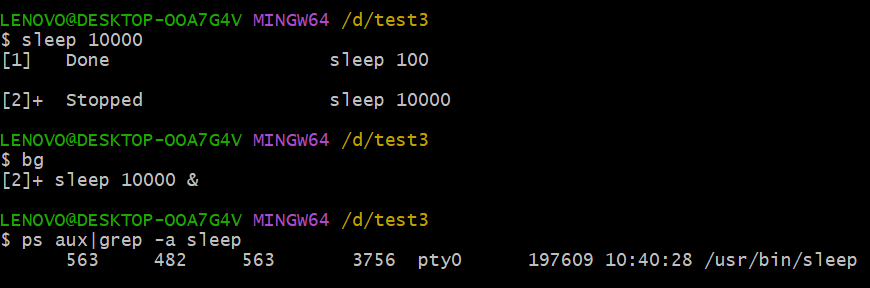
\includegraphics[width = 10cm]{1}
	
	然后应该用pkill命令来删除该进程,但是同样因为Gith(Bash)中没有pkill指令,我便使用了具有相同功能的kill命令来删除,输入kill pid即可。
	
	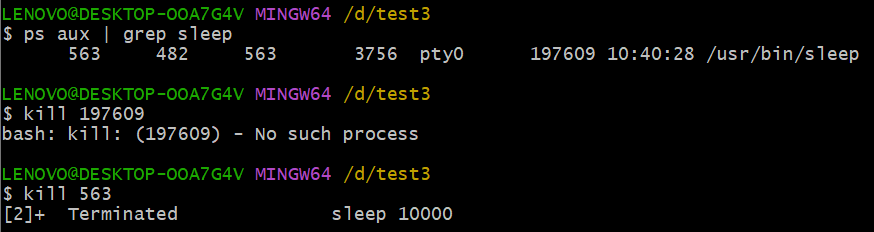
\includegraphics[width = 10cm]{2}
	
	\subsubsection{为您的配置文件新建一个文件夹,并设置好版本控制在其中添加至少一个配置文件,比如说您的 shell,在其中包含一些自定义设置(可以从设置 \$PS1 开始)。}
	首先创建一个gits目录gits目录用来存放所有git及github仓库,然后在gits目录中创建目录dotfiles,用来存放本机的配置文件如 .vimrc/.bashrc/.tmux.conf 等。

	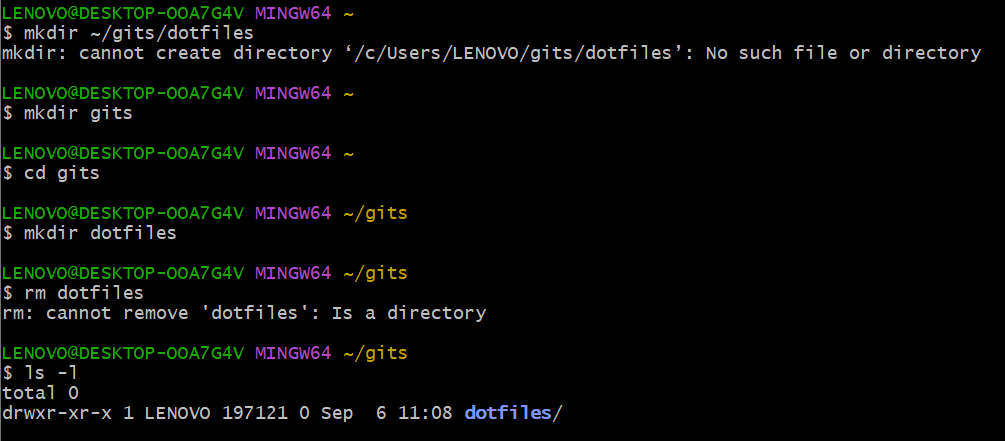
\includegraphics[width = 10cm]{3}

	然后进入dotfiles目录中的master分支,即可查看目录中的相关内容。

	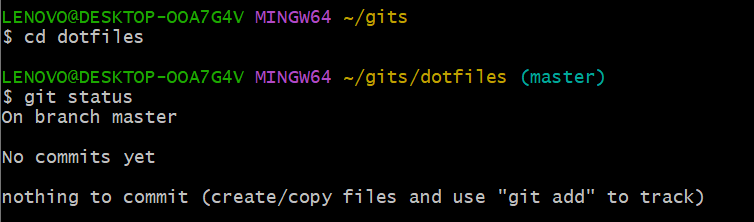
\includegraphics[width = 10cm]{4}
	
	\subsubsection{完成题目所给的tmux教程,并且参考那些步骤来学习如何自定义tmux}
	tmux 是一个终端复用器,它允许用户在一个终端窗口中创建、管理和切换多个会话。使用 tmux,你可以在一个窗口中运行多个会话,并且能够在不同的会话间轻松切换。
	
	该部分内容我校将在我的Linux虚拟机的终端中来完成。首先需要下载、配置tmux的运行环境,在终端中输入命令sudo apt-get install tmux即可开始下载。

	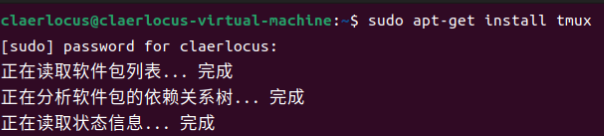
\includegraphics[width = 12cm]{5}

	下载完毕后,在终端中输入命令tmux即可创建窗口。

	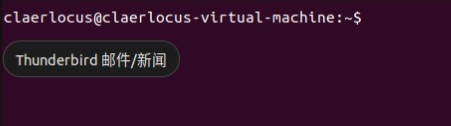
\includegraphics[width = 8cm]{6}

	在tmux窗口中按下Ctrl-b然后按下c即可创建一个新的窗口。
	
	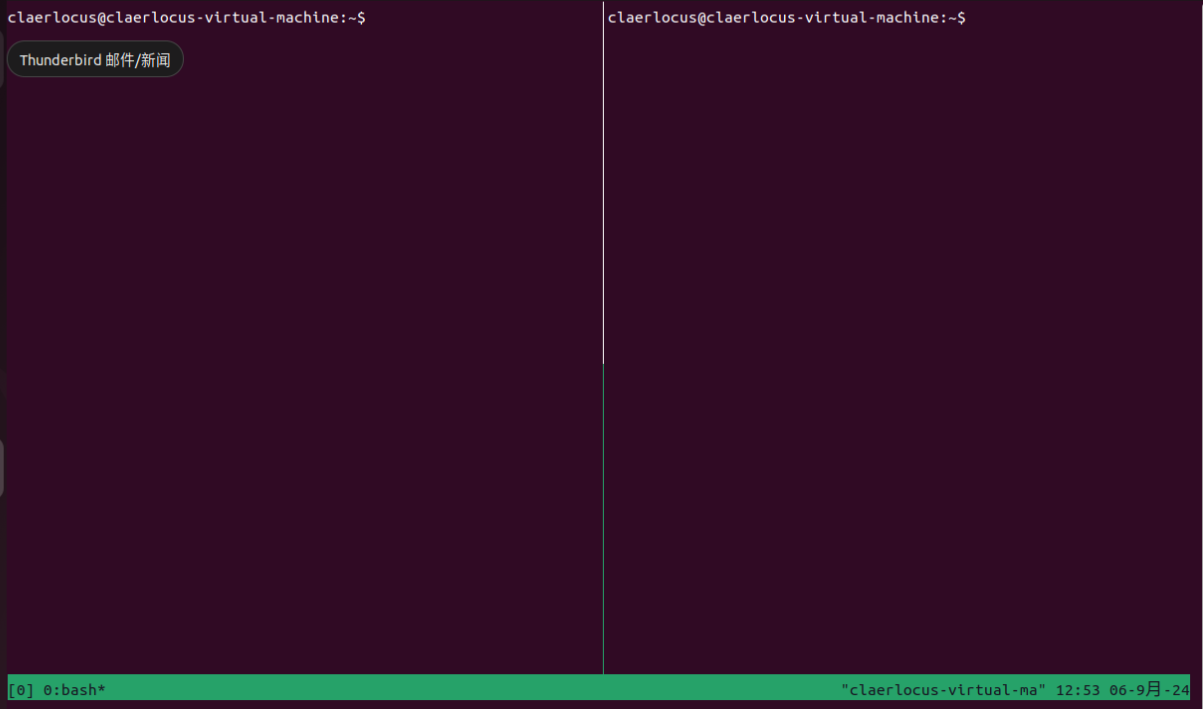
\includegraphics[width = 10cm]{7}
	
	按下Ctrl-b后按n(next)和p(previous)可以让输入光标在两个窗口之间切换。
	
	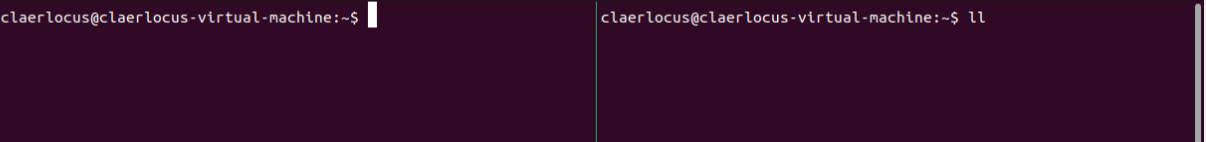
\includegraphics[width = 10cm]{8}
	
	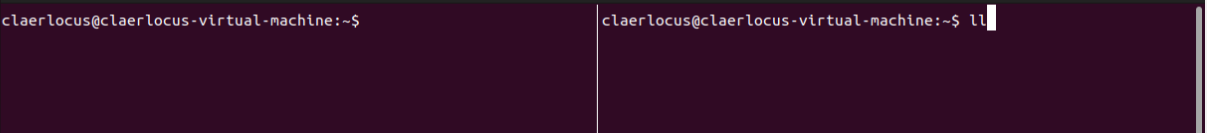
\includegraphics[width = 10cm]{9}
	
	按下Ctrl-b后,再按下d即可关闭并退出当前窗口。
	
	\subsubsection{创建一个 dc 别名,它的功能是当我们错误的将 cd 输入为 dc 时也能正确执行。}
	
	我们需要知道的是创建别名的命令alias,在终端中输入命令alias 原名=别名 即可,在此练习中,我并没有严格按照题目要求将cd改别名为dc,二十将git改为了gt二者其实一模一样。改完后用alias命令查看所有的别名,发现多出了gt。然后用unalise删除别名,完成练习。

	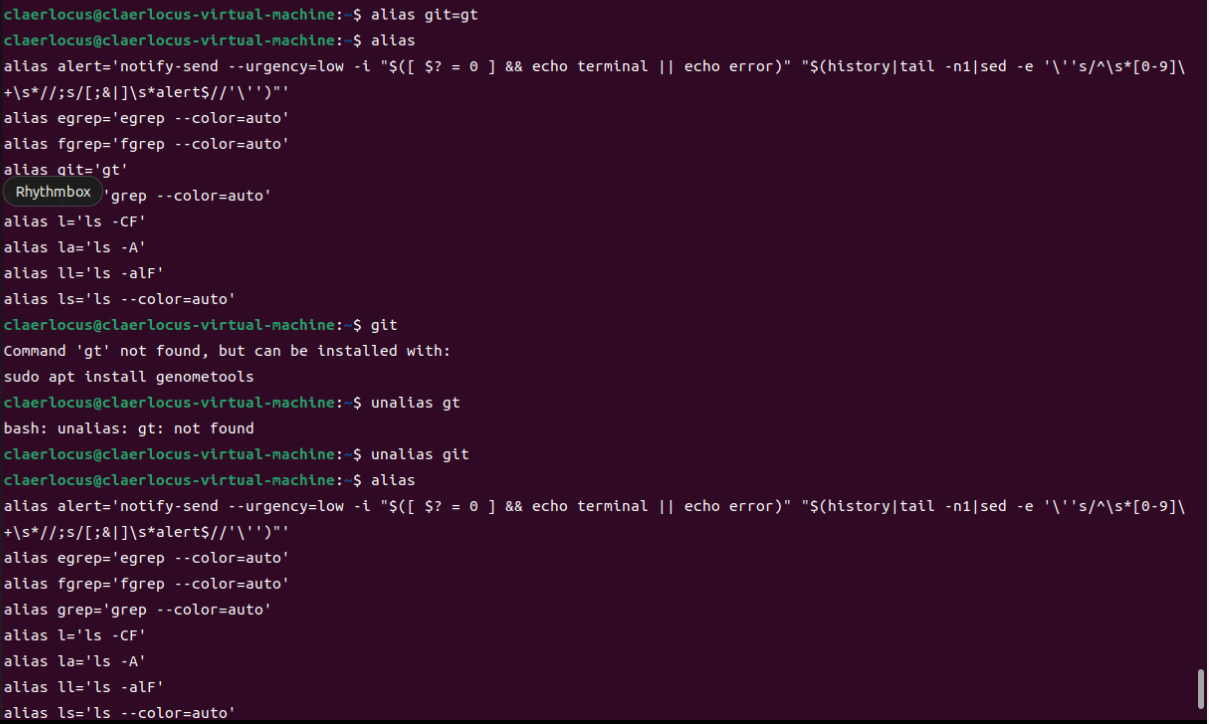
\includegraphics[width = 14cm]{10}

	
	\section{实验中遇到的问题与解决方法}
	\subsection{输入命令pgrep想要获取进程的pid时,显示该命令是无效的命令}

	这是因为pgrep命令是ps aux | grep命令的缩写,然而在Git(Bash)中并没有相关的缩写,想要获取进程的pid应该完整地输入命令ps aux | grep。并且加上-a或者-f来详细说明要求。
	
	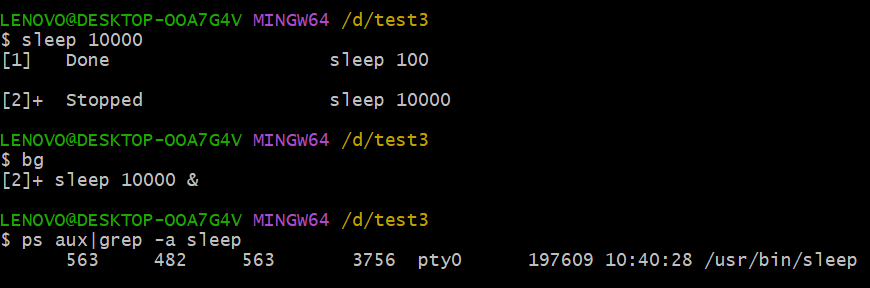
\includegraphics[width = 10cm]{1}
	
	\subsection{在Linux系统的虚拟机终端上输入python查看python版本时,显示该命令无效}
	
	在终端中下载的python版本为python3,输入python3可以查看python版本,想要使用python命令来查看python版本应该将python3与python绑定,解决方法如下图所示。
	
	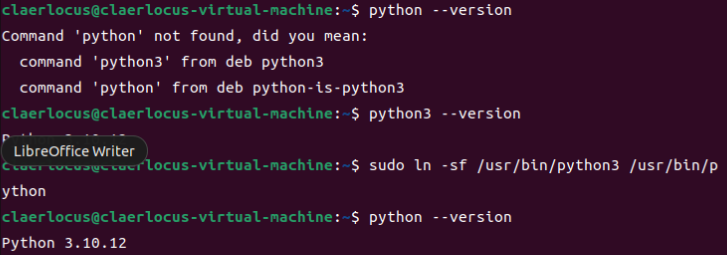
\includegraphics[width = 10cm]{11}

	\subsection{在bash中想用pkill命令来删除进程,但是却无法删除}
	
	Bash中没有pkill命令,但是有相同用法以及作用的kill命令,使用kill pid即可删除相应的进程。
	
	\section{实例练习}
	\subsection{使用python写一段程序,计算两个数的和}
	代码与运行结果如下:

	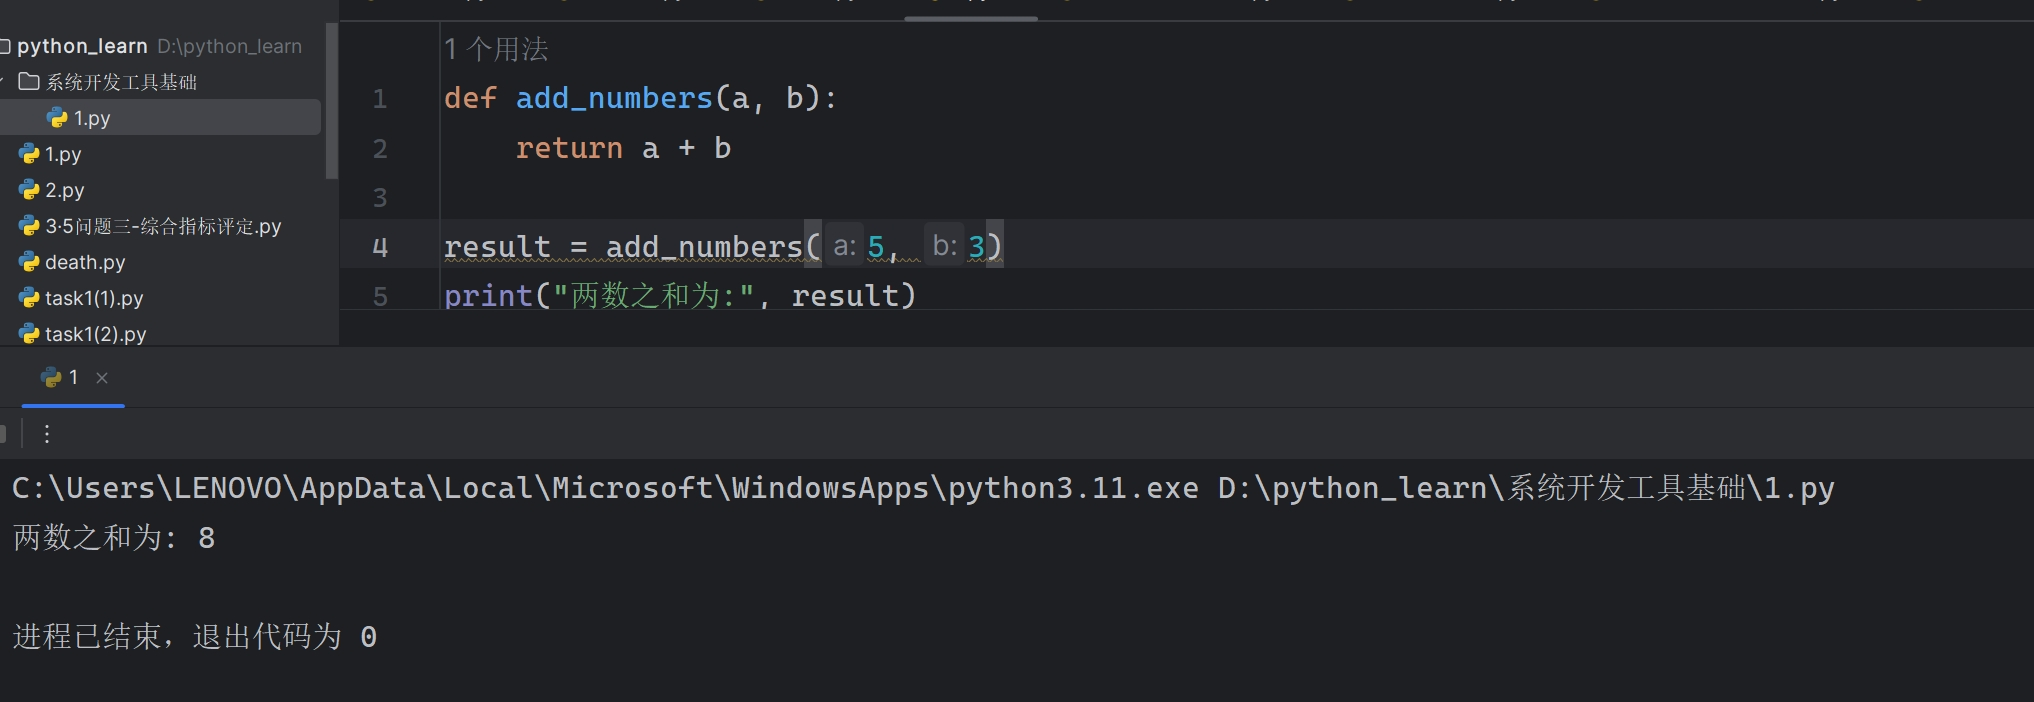
\includegraphics[width = 16cm]{12}
	
	\subsection{使用python写一段程序,判断一个数是否为素数}
	素数即为因子只有1和它本身的数,判断一个属是否为素数书即看他能否被除了1和它本身之外的数整除,代码与运行结果如下:

	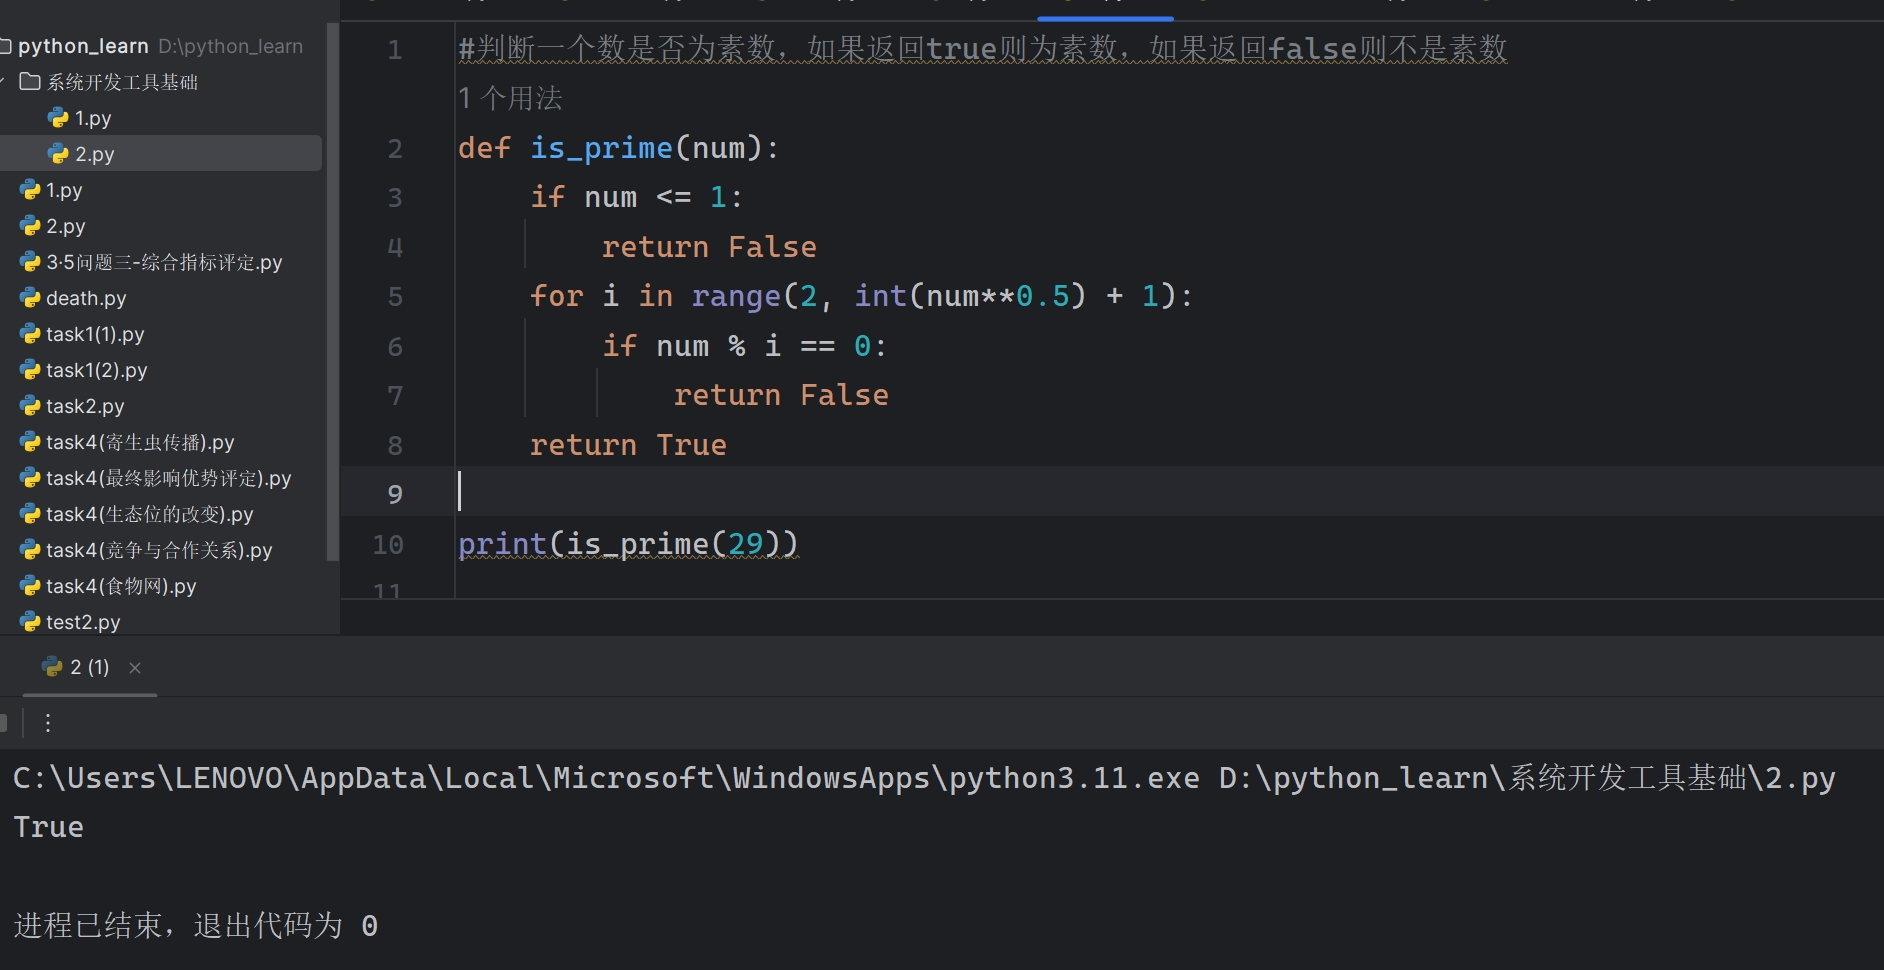
\includegraphics[width = 16cm]{13}

	\subsection{使用python写一段程序,打印出斐波那契数列的前n项}
	斐波那契数列指第一项是0.第二项是1,之后的每一项都是它前两项的和的一列数,求其前n项的代码和运行结果如下:
	
	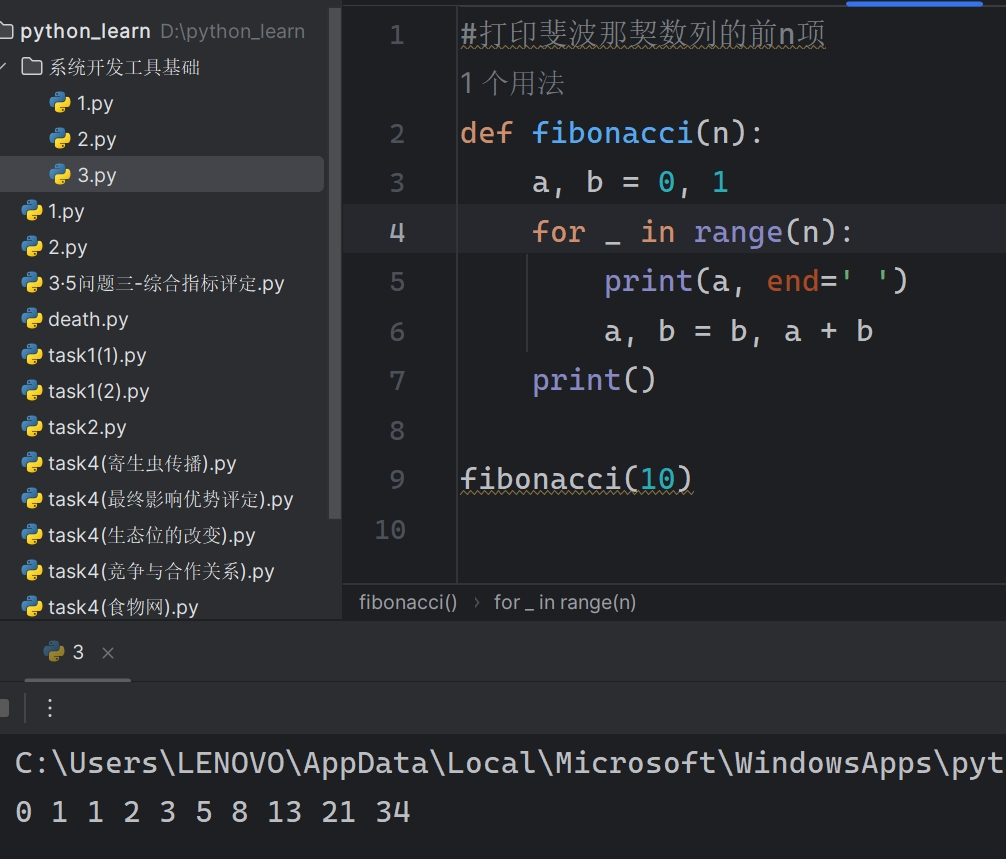
\includegraphics[width = 14cm]{14}
	
	\subsection{使用python写一段程序,实现字符串反转功能}
	定义 reverse\_string 的函数,接受一个字符串 s 后返回这个字符串的反转,通过 s[::-1] 实现,其中 [::-1] 是一个字符串的切片操作,用于将字符串倒序排列。
	
	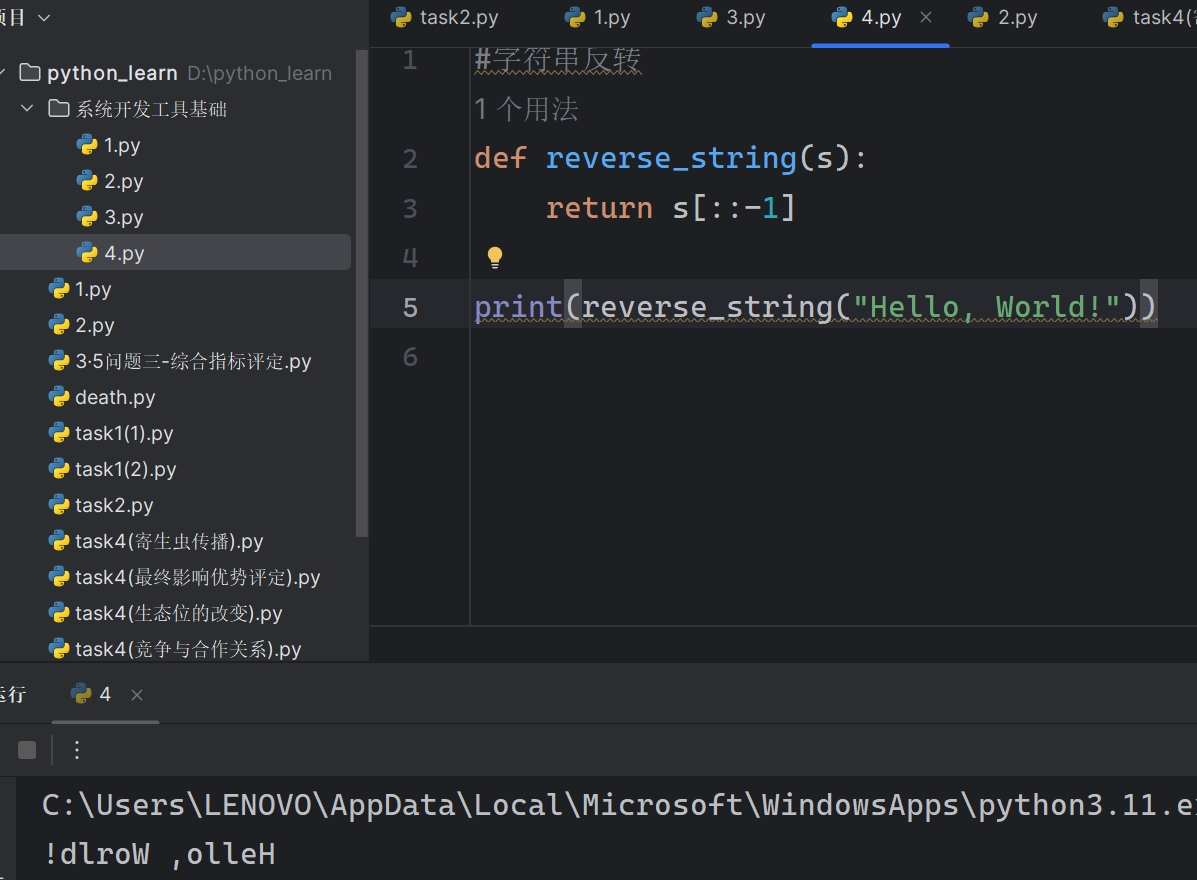
\includegraphics[width = 14cm]{15}
	
	
	\subsection{使用python写一段程序,实现字符串反转功能}
	定义一个函数average,用于接受一个列表作为参数之后,计算列表数的平均值,需要用到python中列表本身包含的函数——sum(加和函数)、len(列表长度函数)。
	
	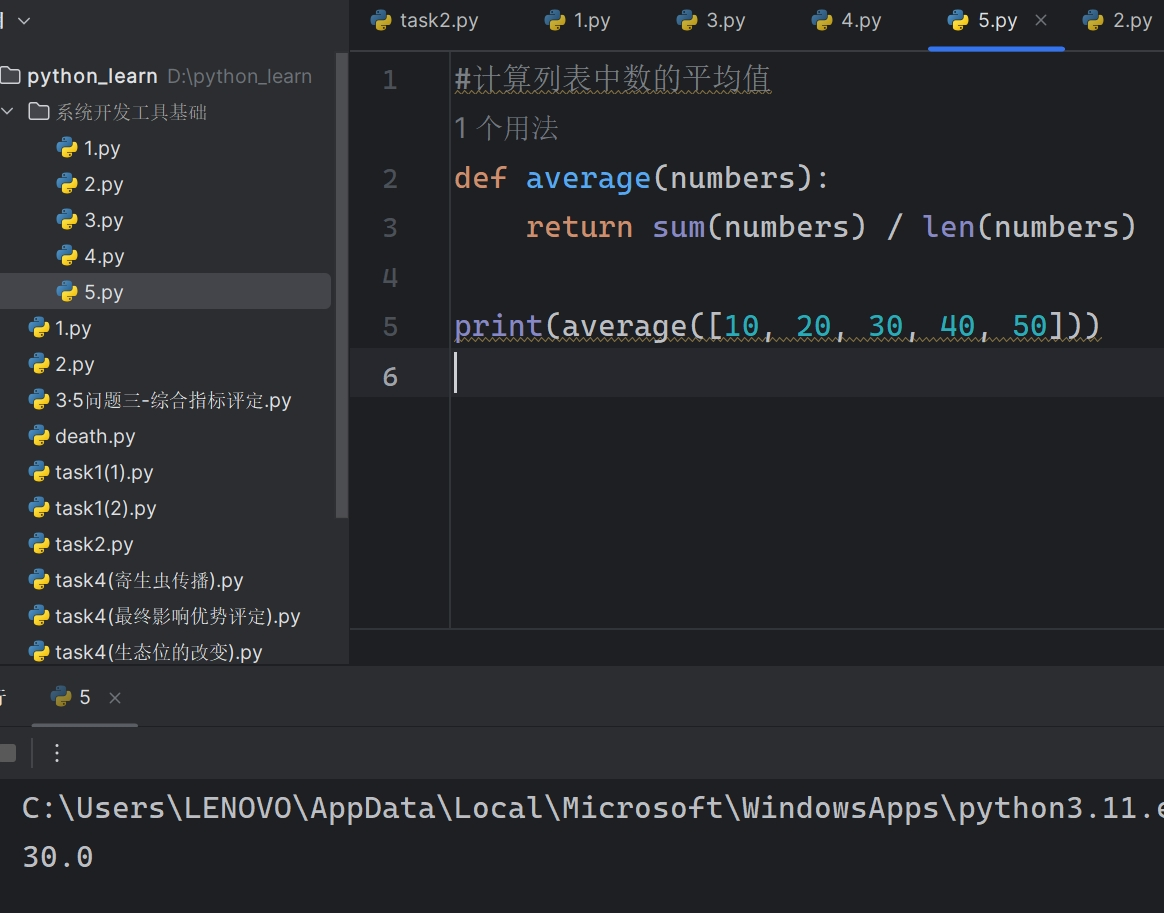
\includegraphics[width = 14cm]{16}
	
	\subsection{判断一段字符串是否为回文}
	利用字符串反转函数,判断反转后的字符串和反转前的字符串是否相同,相同返回true,不相同返回false。
	
	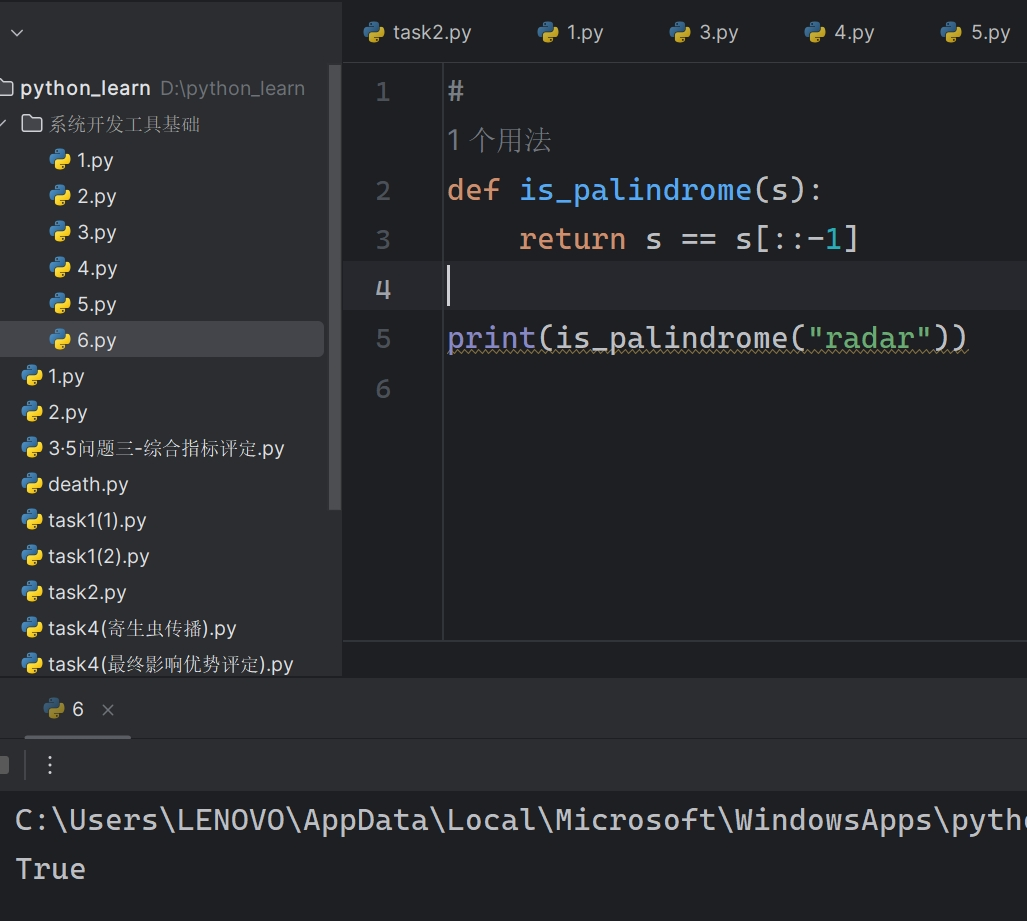
\includegraphics[width = 14cm]{17}
	
	\subsection{读取文件中内容并将其打印出来}
	首先利用open操作打开目标文件(注意目标文件必须与python文件再同一目录中),然后利用read功能读取文件内容,并用print语句将其打印出来。
	
	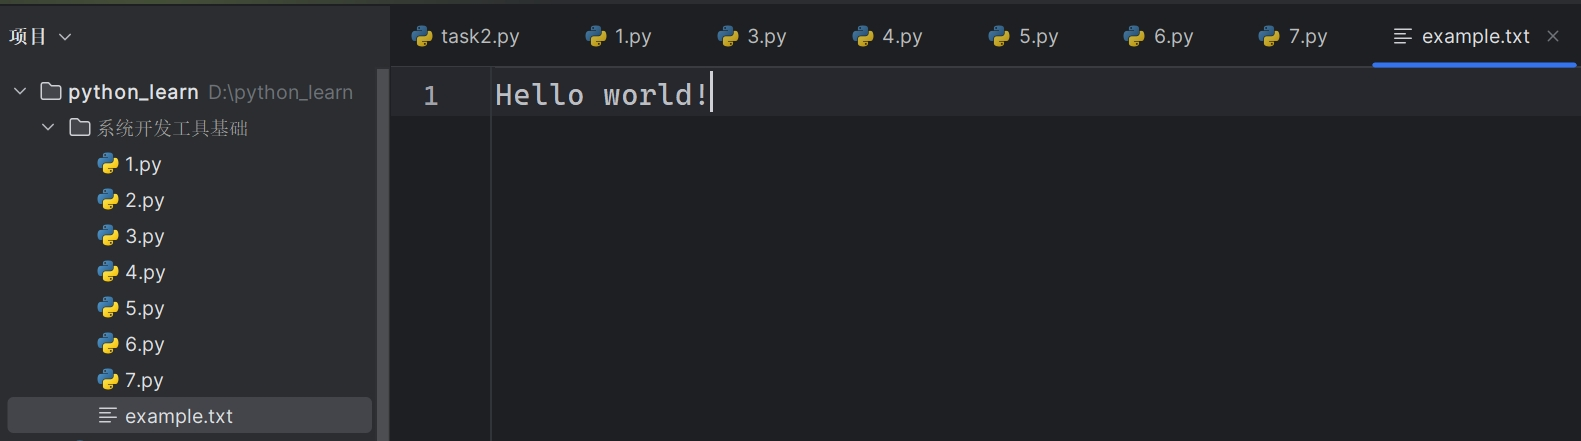
\includegraphics[width = 16cm]{18}
	
	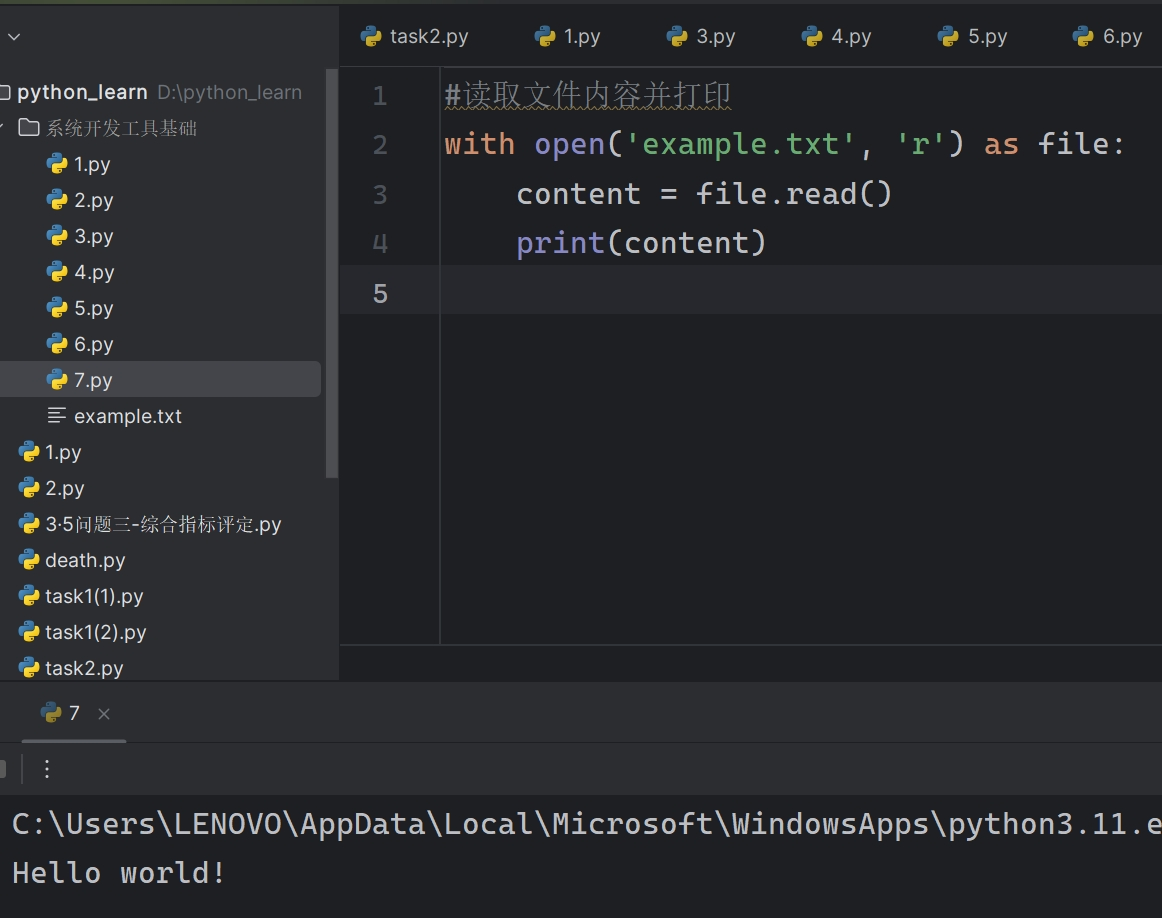
\includegraphics[width = 14cm]{19}
	
	\subsection{利用递归实现快速排序算法}
	用python编写一个程序,使用递归算法对一个列表中的数字进行快速排序。
	
	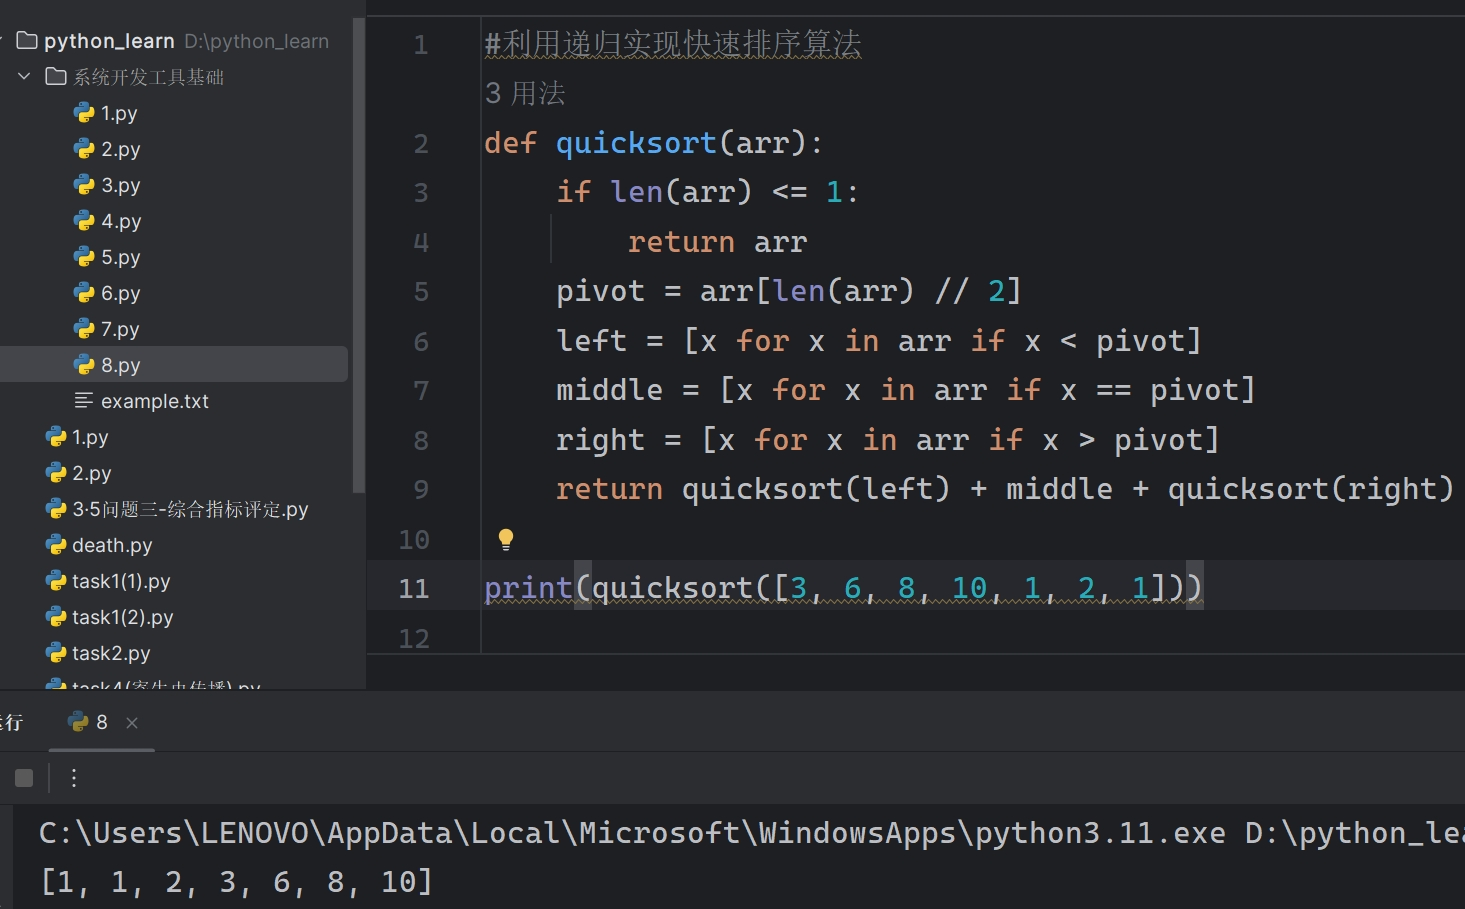
\includegraphics[width = 14cm]{20}
	
	\subsection{引入turtle库进行简单的图像绘制}
	首先引入turtle库,然后设置三个同心圆的半径与颜色,最后再进行绘制。
	
	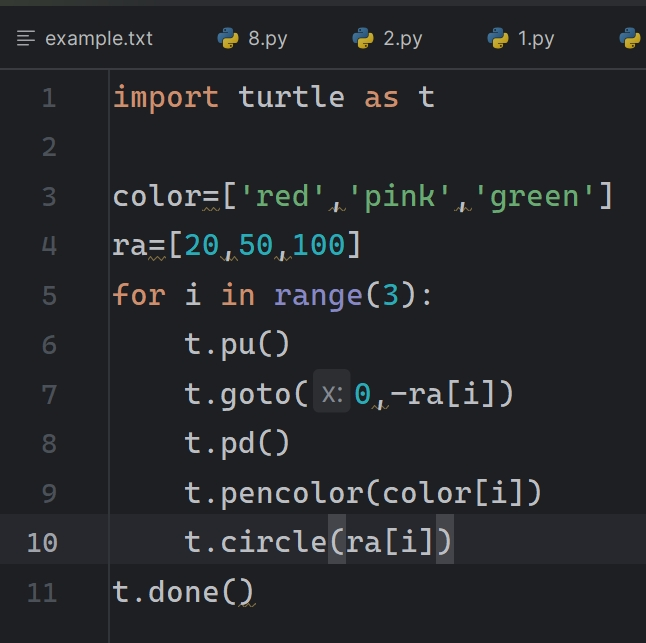
\includegraphics[width = 10cm]{21.1}
	
	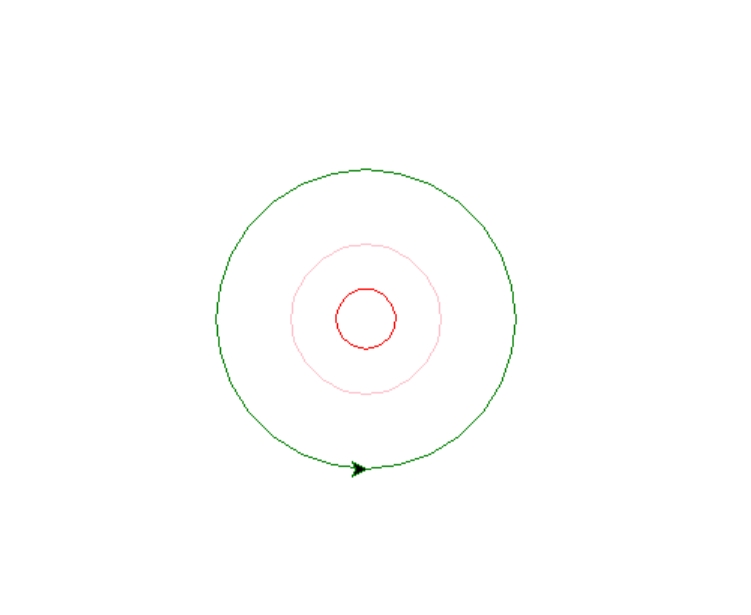
\includegraphics[width = 10cm]{21.2}
	
	\subsection{使用matplotlib绘制正弦波形}
	想要绘制正弦波形需要引入numpy库,和matplotlib库中的pyplot库。具体代码与绘制结果如下:
	
	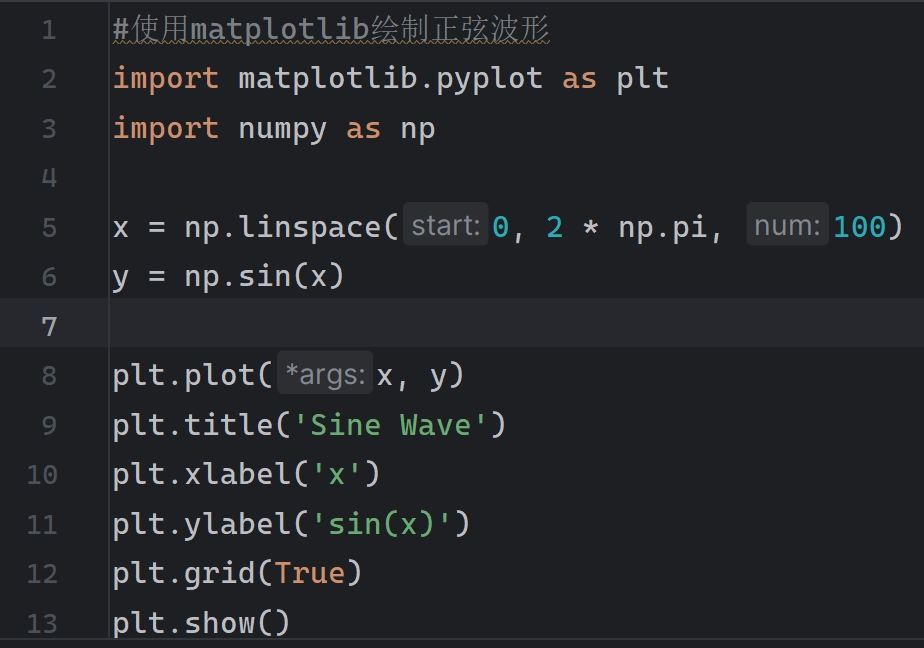
\includegraphics[width = 10cm]{22.1}
	
	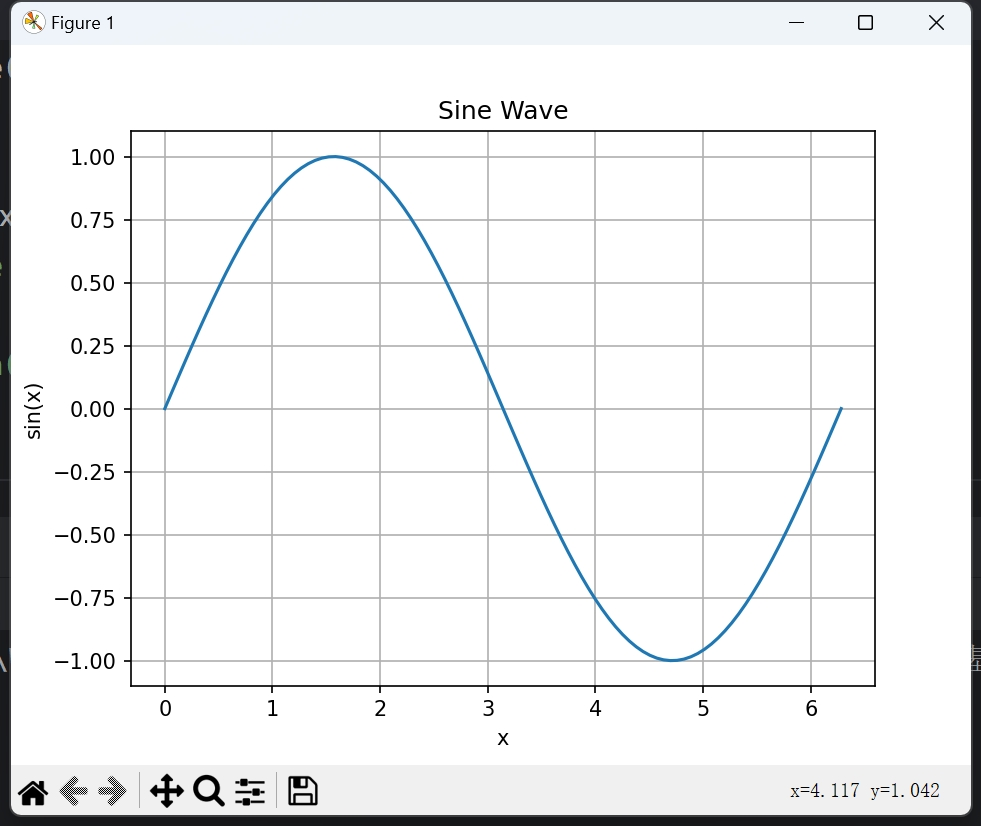
\includegraphics[width = 10cm]{22.2}
	
	\subsection{使用Tkinter创建一个简单的图形用户界面}
	引入tkinter库,据同日代码与运行效果如下:
	
	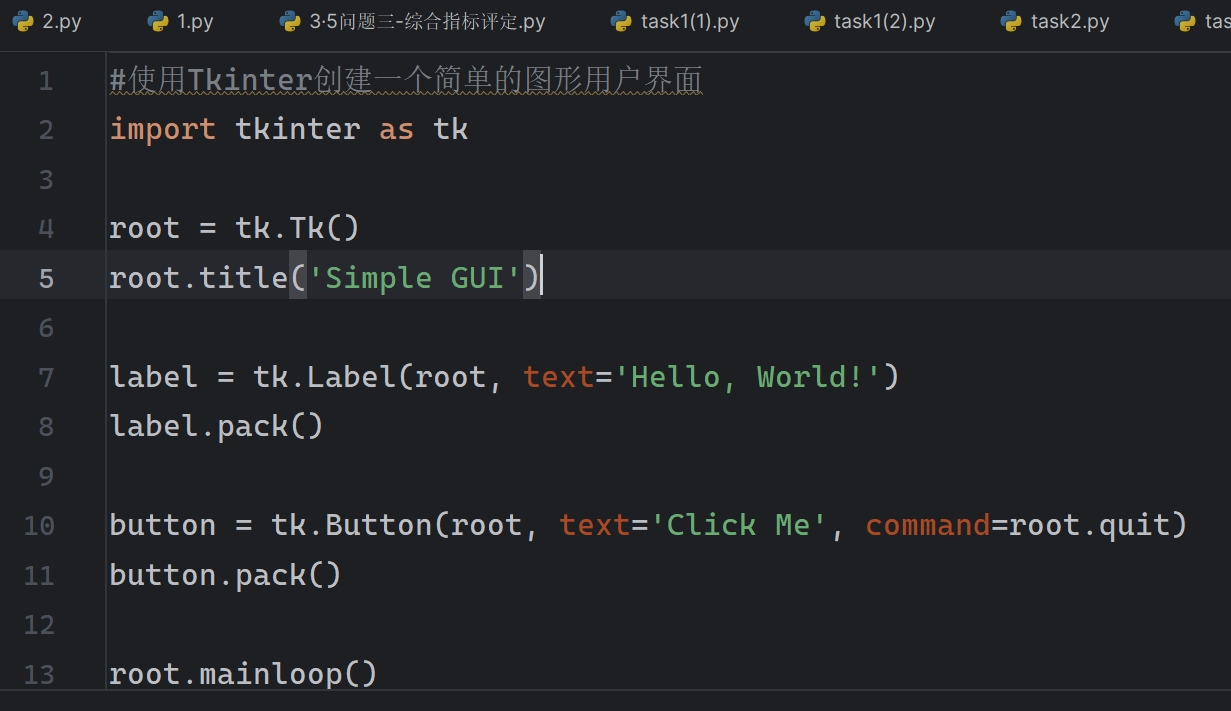
\includegraphics[width = 14cm]{23.1}
	
	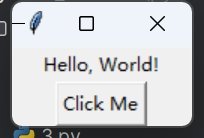
\includegraphics[width = 8cm]{23.2}
	
	\subsection{暂停一秒输出}
	使用 time 模块的 sleep() 函数。
	
	
	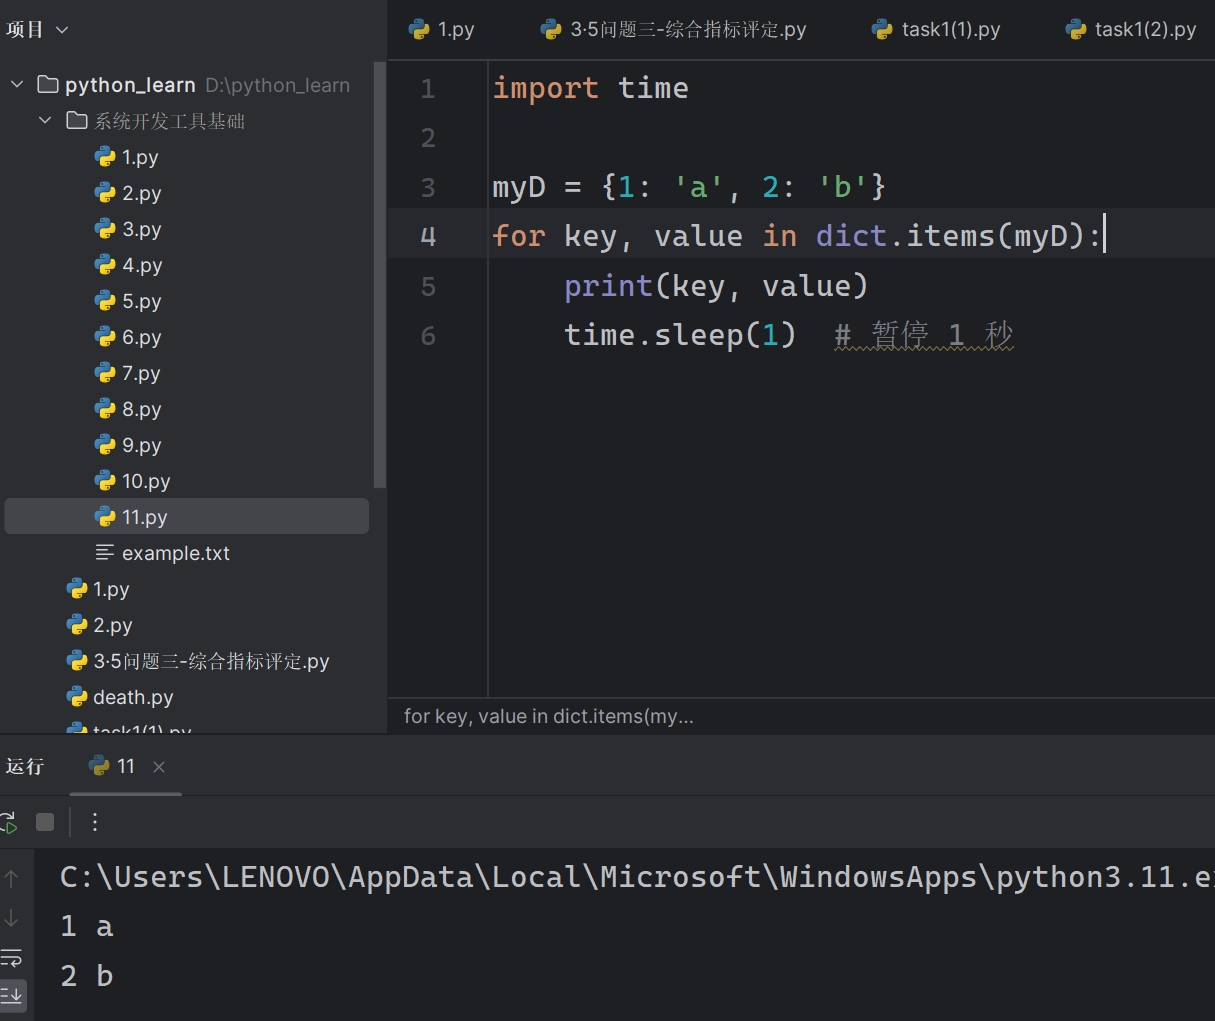
\includegraphics[width = 14cm]{24}
	
	\subsection{打印出所有的"水仙花数"}
	所谓"水仙花数"是指一个三位数,其各位数字立方和等于该数本身。利用for循环控制100-999个数,每个数分解出个位,十位,百位。
	
	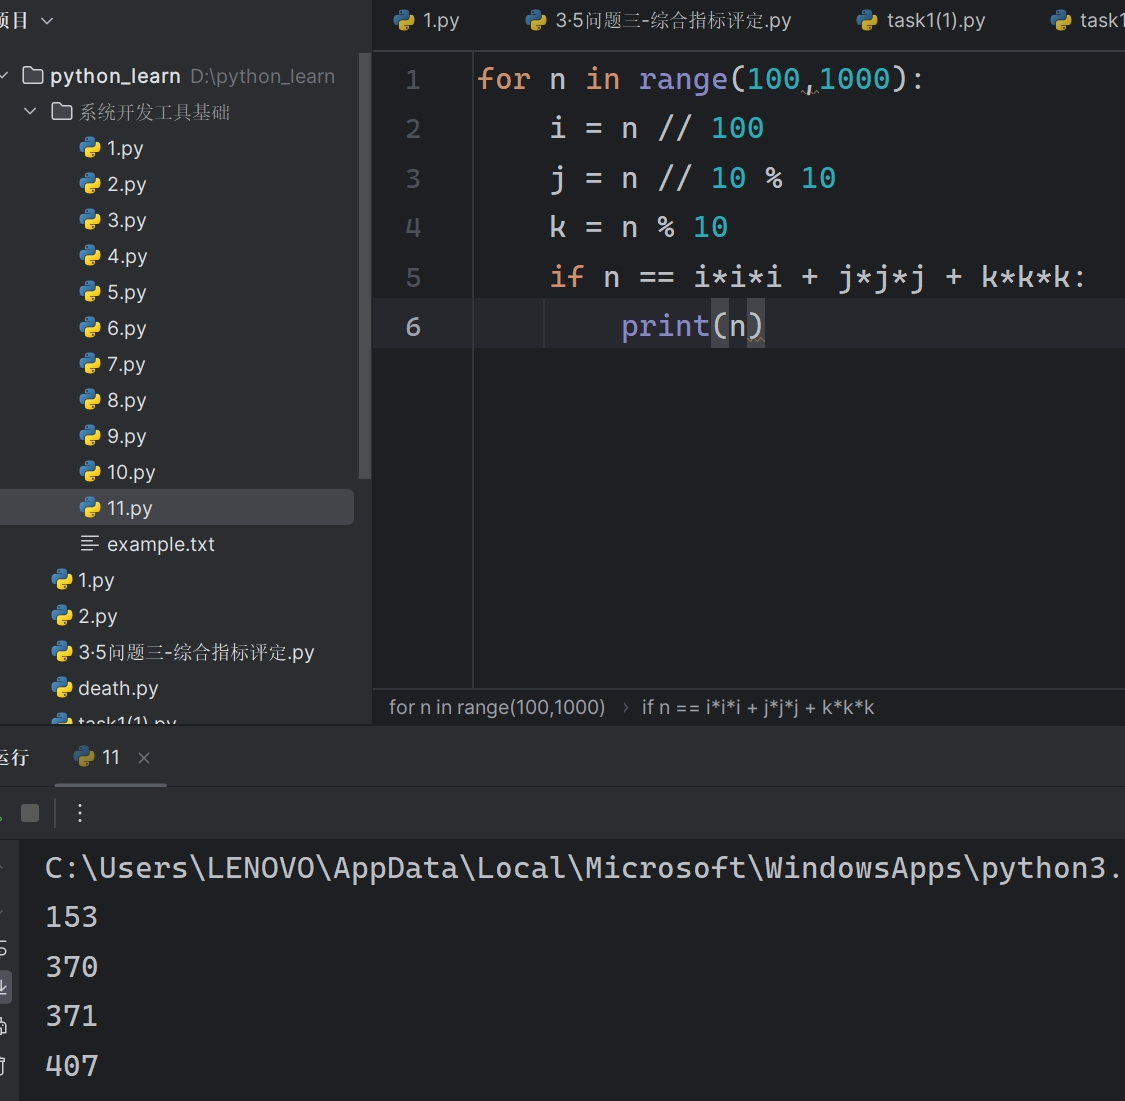
\includegraphics[width = 14cm]{25}
	
	\subsection{输出指定格式的日期}
	使用 datetime 模块。
	
	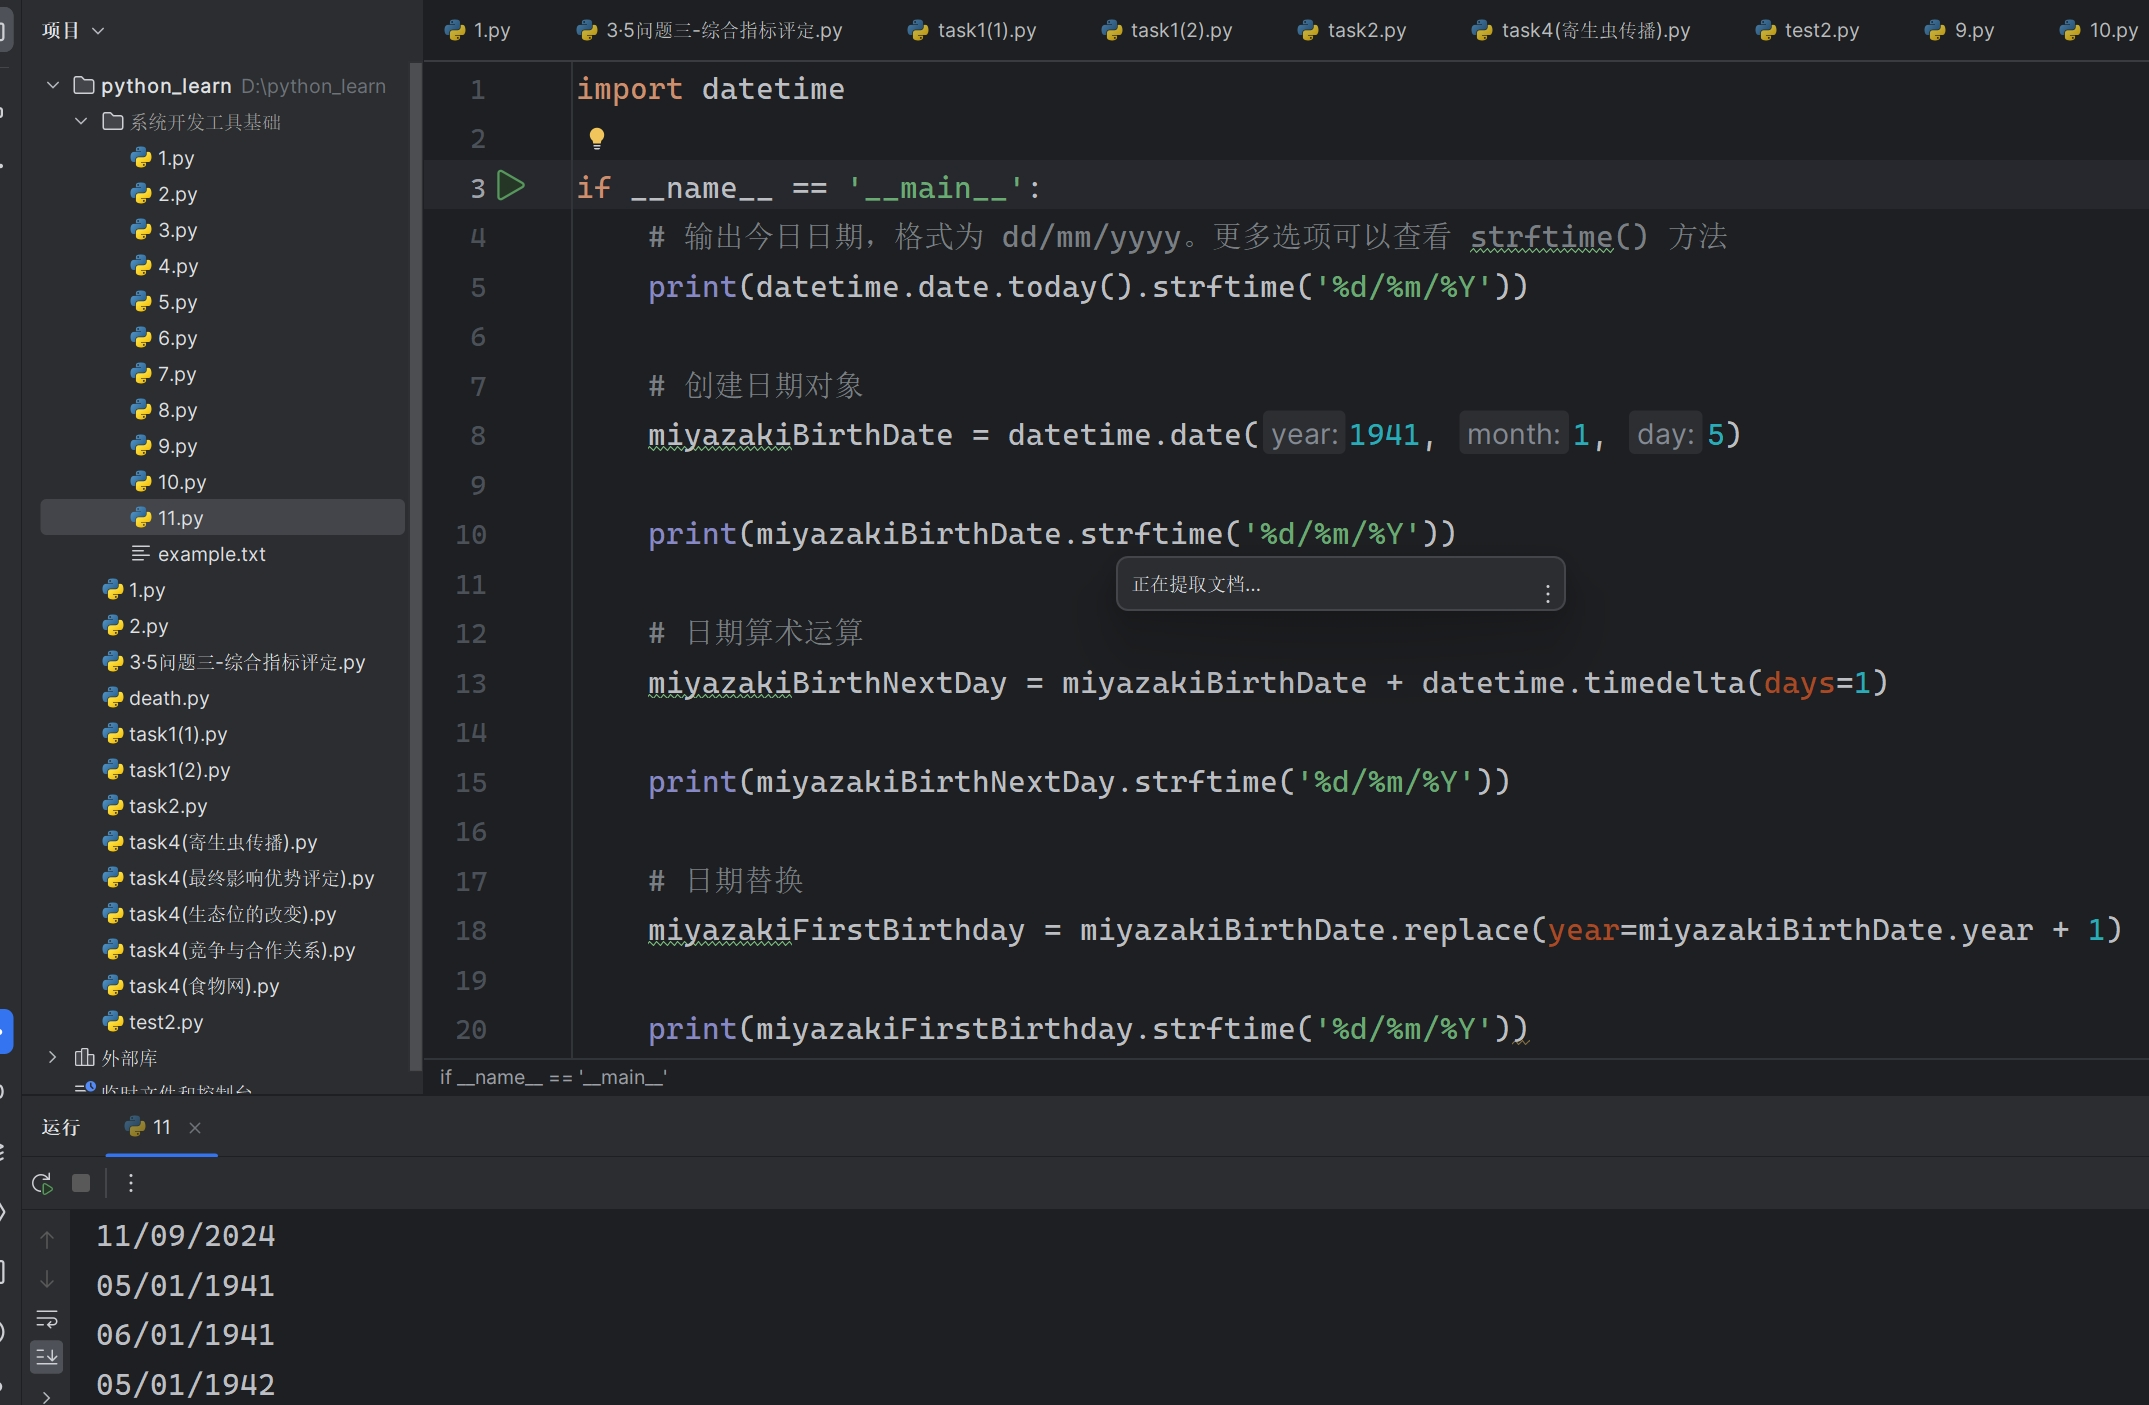
\includegraphics[width = 16cm]{26}
	
	\subsection{输入一行字符,分别统计出其中英文字母、空格、数字和其它字符的个数。}
	利用 while 或 for 语句,条件为输入的字符不为回车符。
	 
	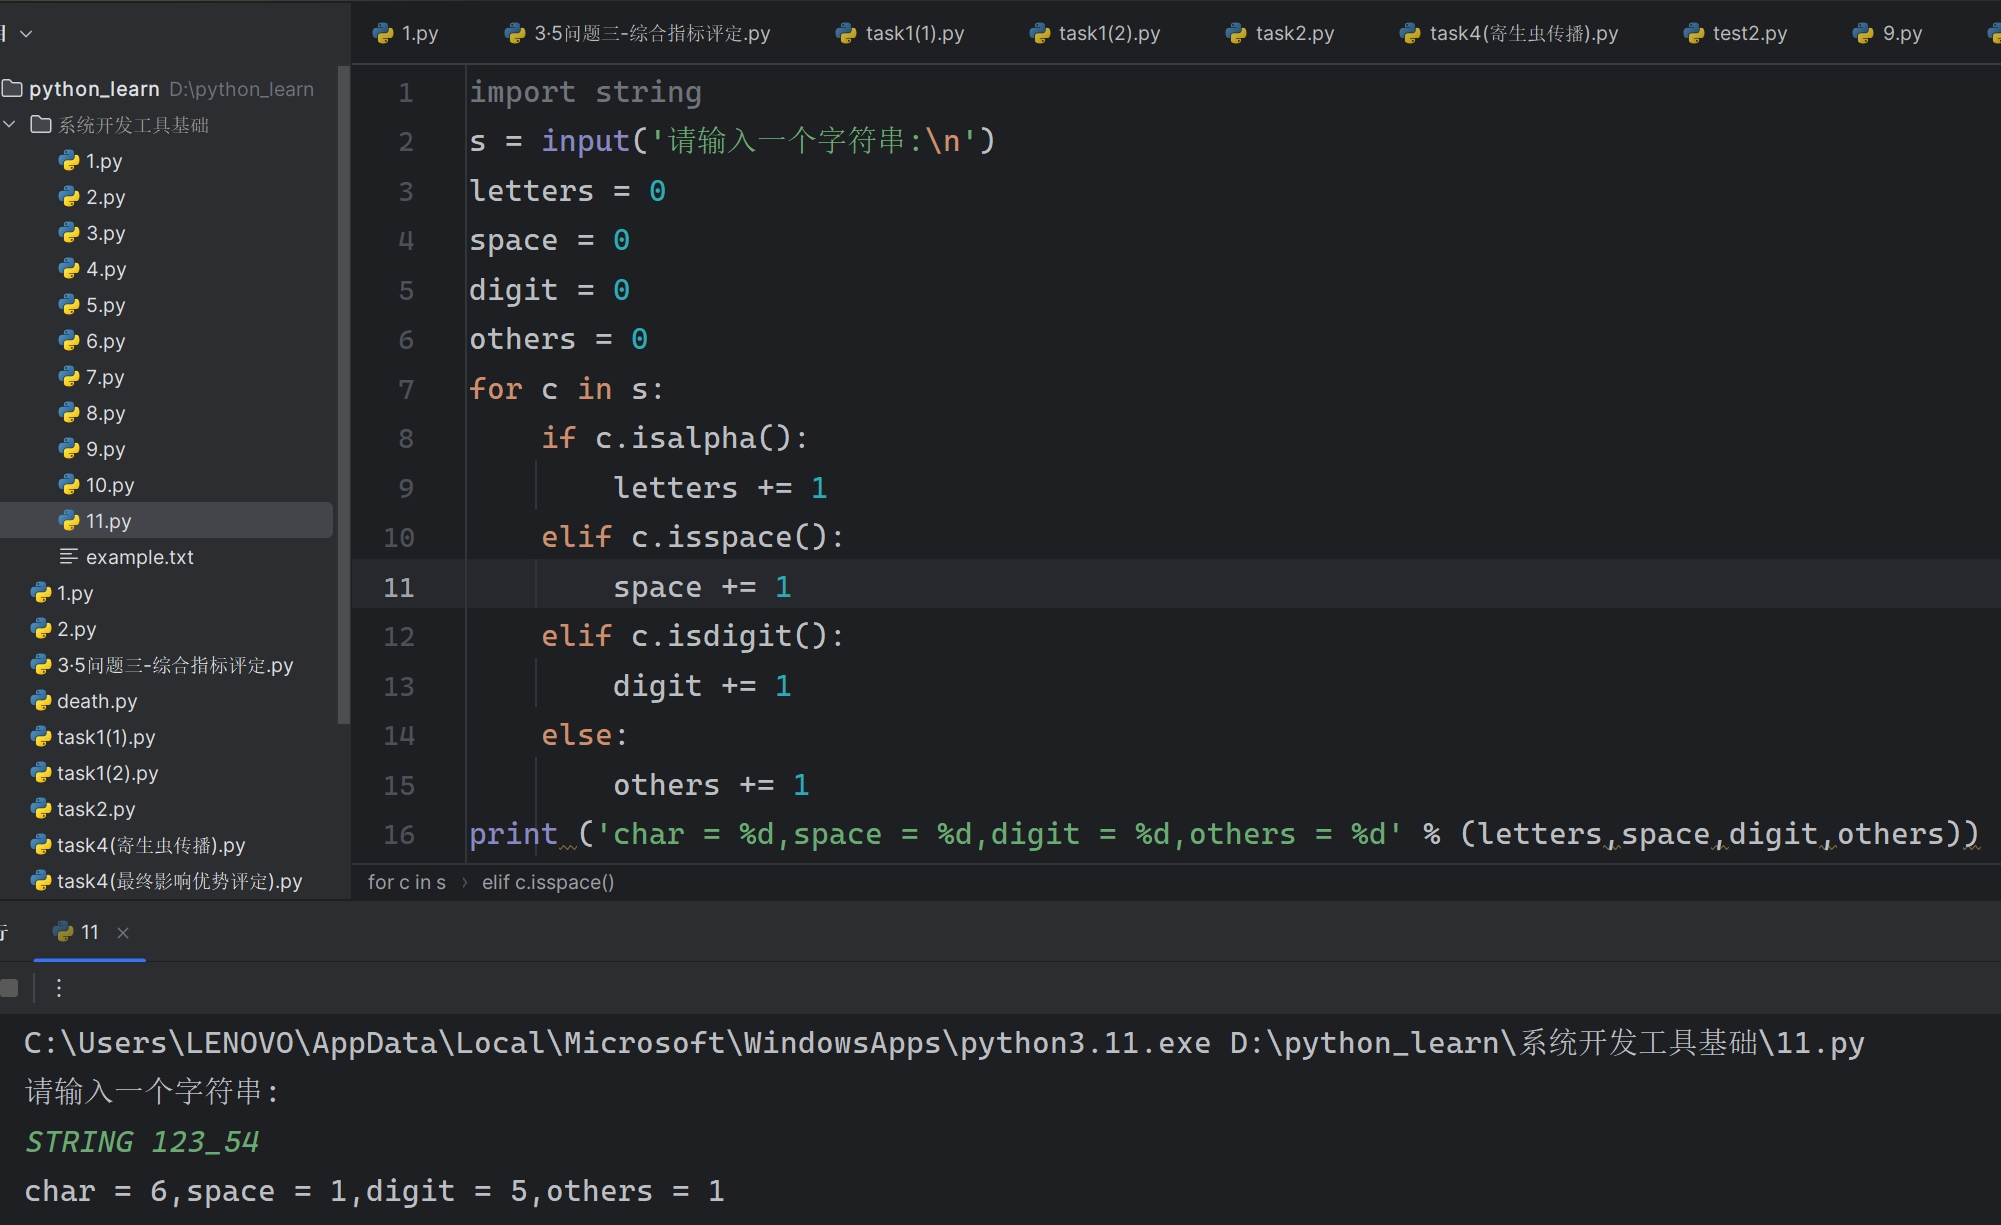
\includegraphics[width = 14cm]{27}
	
	\subsection{绘制一个简单的食物网}
	该实例需要导入第三方库networkx,来创建有向图,然后写入数据,将有向图连接,修改绘图样式。
	
	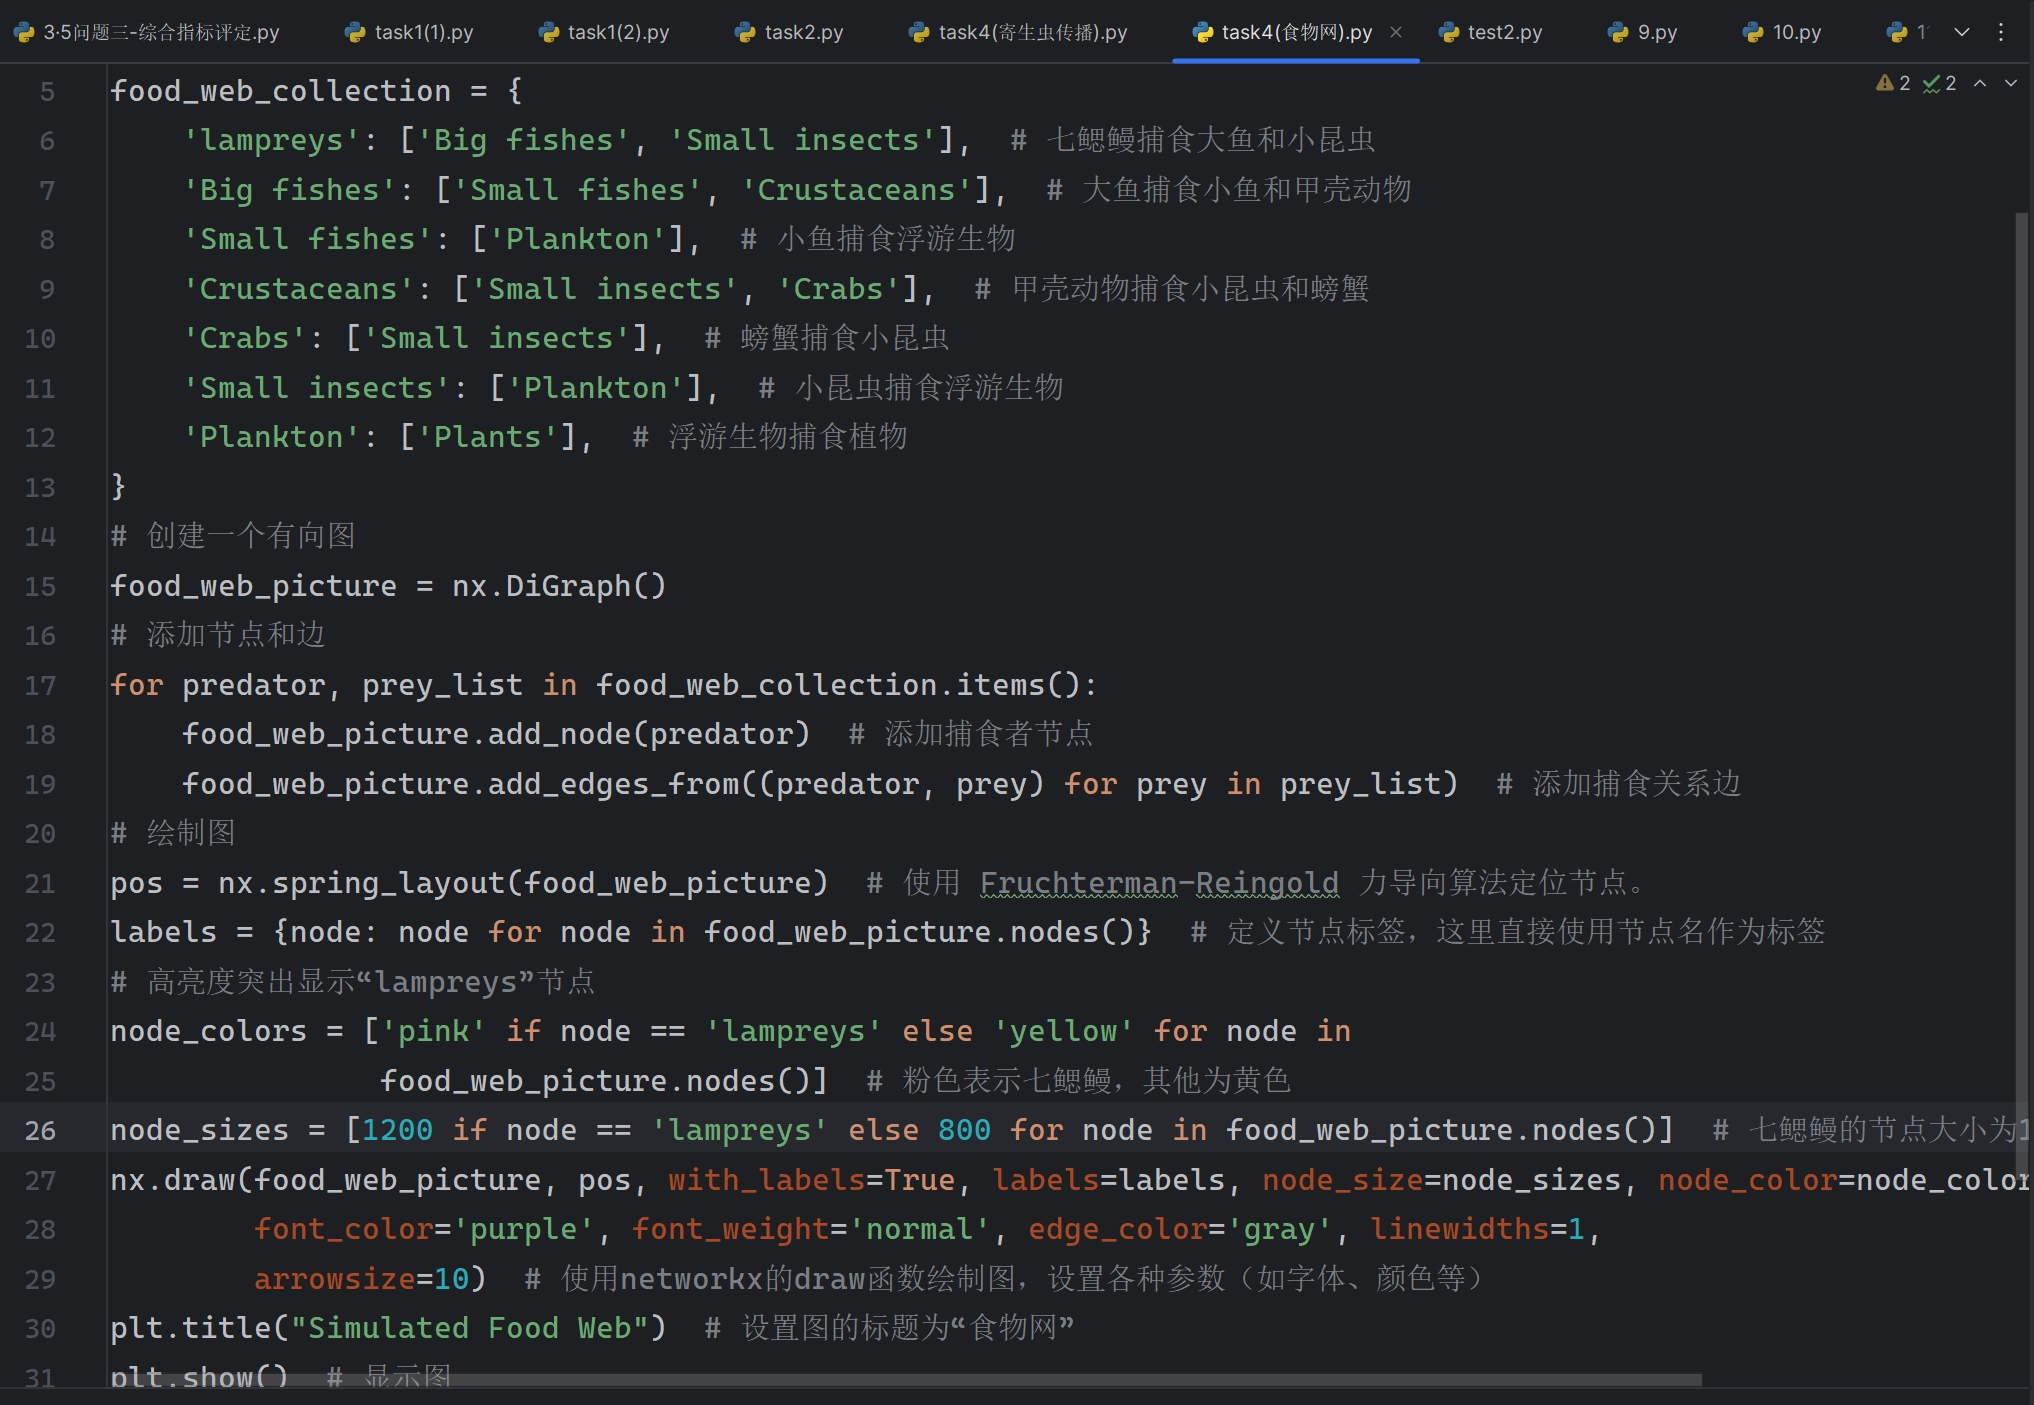
\includegraphics[width = 18cm]{28.1}
	
	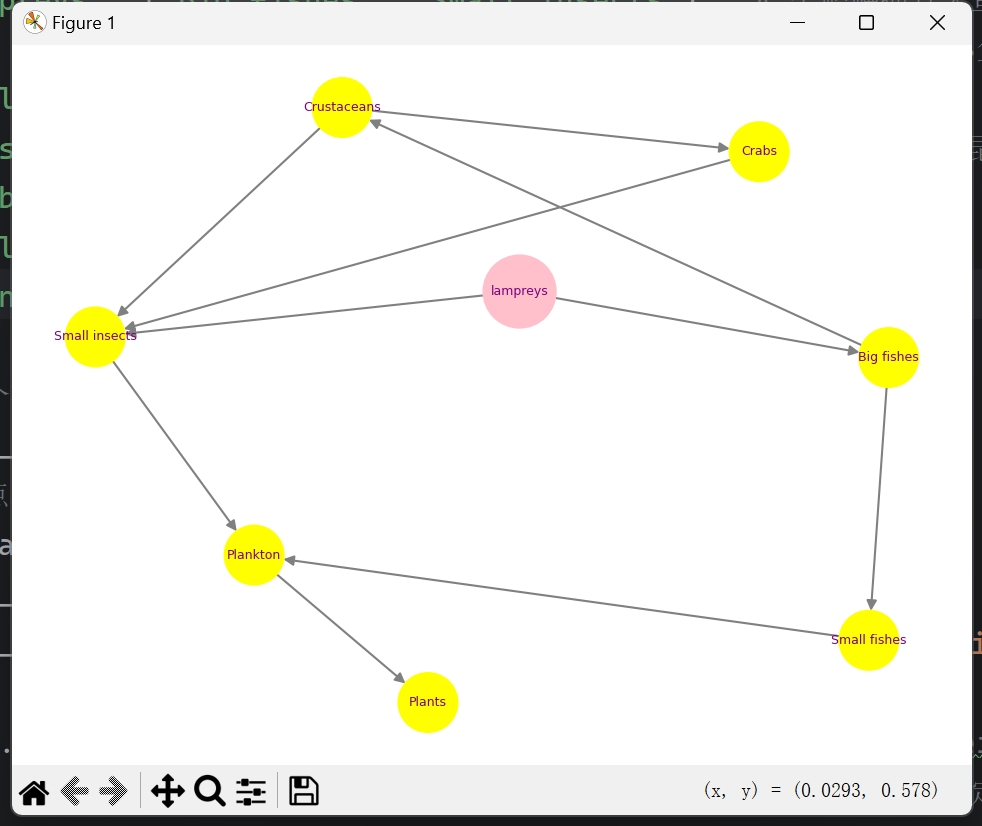
\includegraphics[width = 14cm]{28.2}
	
	\subsection{写一个计时器}
	
	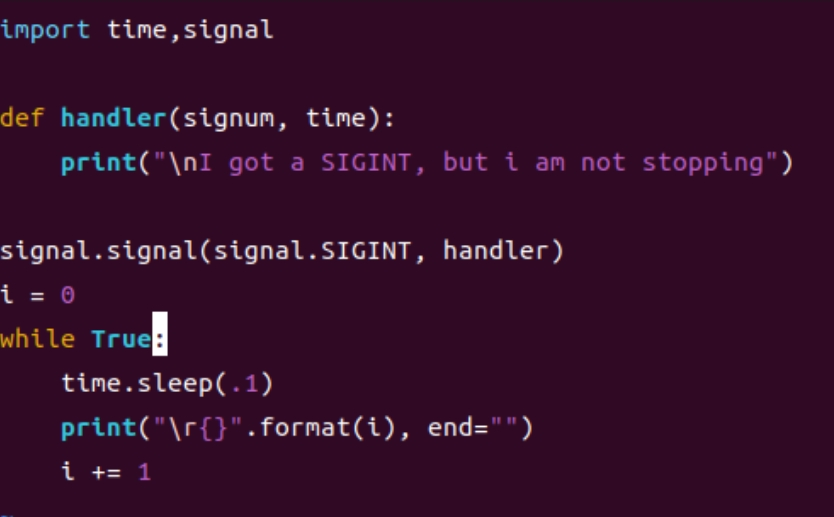
\includegraphics[width = 12cm]{29.1}
	
	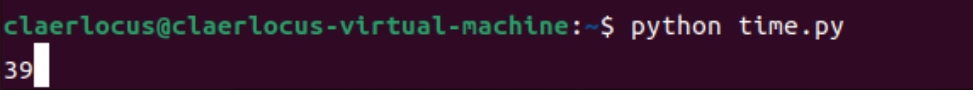
\includegraphics[width = 12cm]{29.2}
	
	
	\subsection{写一个简易加法计算器}
	
	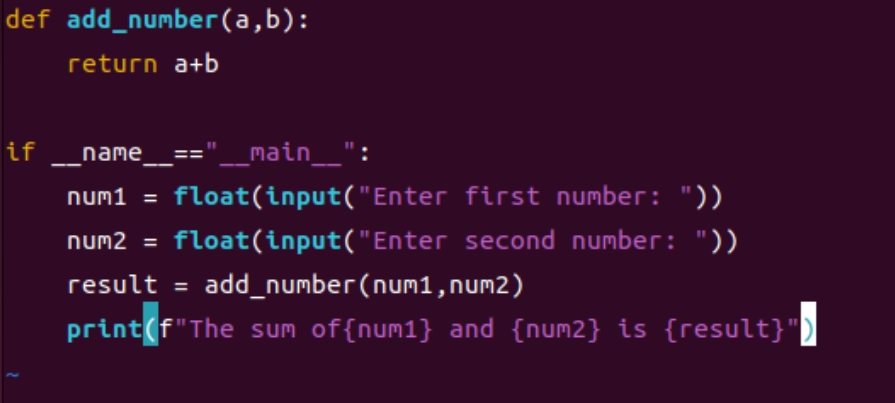
\includegraphics[width = 12cm]{30.1}
	
	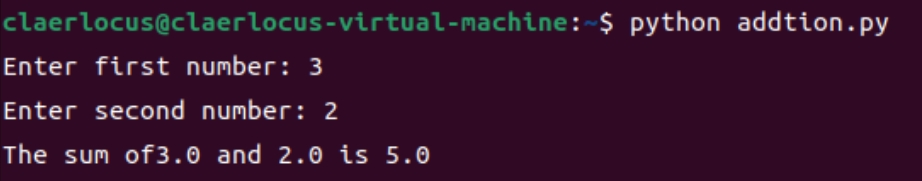
\includegraphics[width = 12cm]{30.2}
	
	\subsection{文件列表器}
	
	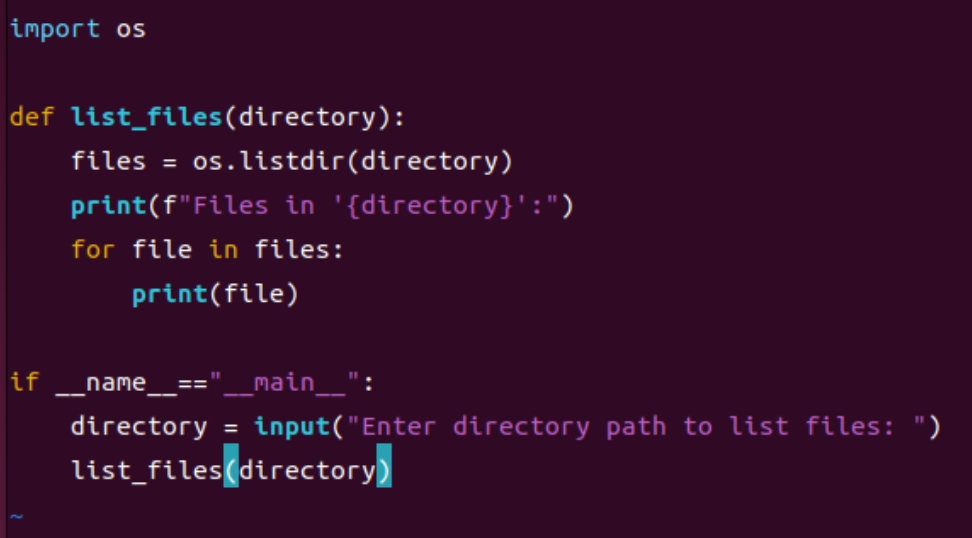
\includegraphics[width = 12cm]{31.1}
	
	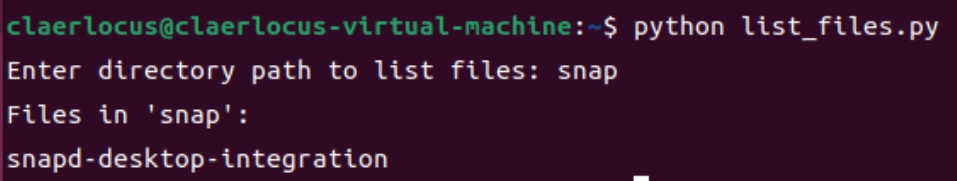
\includegraphics[width = 12cm]{31.2}
	
	\subsection{制作一个简单的HTTP服务器}
	
	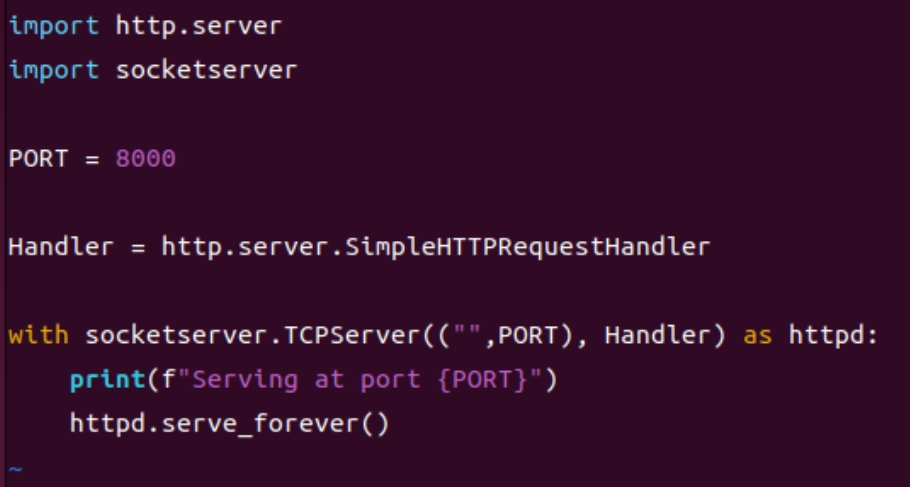
\includegraphics[width = 12cm]{32.1}
	
	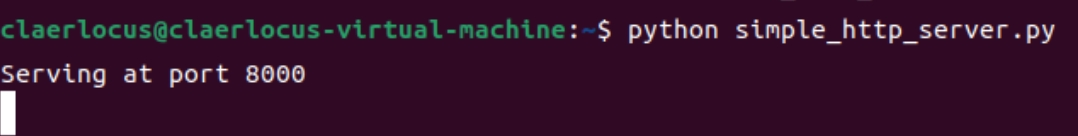
\includegraphics[width = 12cm]{32.2}
	
	\section{实验收获与感悟}
	在深入掌握命令行环境的过程中,我惊喜地发现工作效率得到了显著提升,能够通过编写脚本自动化处理繁琐任务,极大地减少了重复劳动。同时,这种学习经历让我对操作系统有了更深刻的理解,能够在不同操作系统间自如切换,为我打开了一条通往系统管理和高级操作技能的道路。
	
	Python语言的学习之旅让我掌握了这门语言的基础,同时,Python的简洁性和强大的库支持让我能够迅速将想法转化为实际代码,极大地加快了项目的开发进程。此外,得益于Python社区的繁荣,我得以在遇到难题时快速找到解决方案,这也让我感受到了开源文化的力量。
	
	在探索Python视觉应用时,我感受到了技术创新的魅力,体会到了科技的强大了力量,并提升了跨学科解决问题的能力。
	
	整个学习历程是一段丰富而深刻的个人成长之旅。它不仅提高了我的技术能力,更锻炼了我的逻辑思维和解决复杂问题的能力。同时,这一过程也让我认识到,在技术日新月异的今天,持续学习和实践是保持竞争力的关键。我将继续拥抱变化,不断探索新技术,以实现自我超越和技术创新。
	
	Github仓库链接:https://github.com/Locusclaer/-.git
	
\end{sloppypar}
\end{document}